\chapter{Applications}
The main purpose of this work, which is to present \textsc{CosmoLIME}, has been achieved with the conclusion of the previous chapter: we explained in detail why \textsc{CosmoLIME} can aid the task of accelerating cosmological inferences, the tools required to establish such a framework, and how all of these topics converge into how \textsc{CosmoLIME} works internally and is accessed. As a consequence this work is in a sense complete; no further chapters are needed to explain \emph{how} \textsc{CosmoLIME} works or \emph{why} it may be useful. 

We argue that this discussion is actually incomplete; to gain a definitive insight about \textsc{CosmoLIME} some practical applications are needed. Seeing how \textsc{CosmoLIME} works \emph{in practice} is the definitive proof that the new approach to emulation built into \textsc{CosmoLIME} is not only an interesting novelty, but a practical tool with many potentially useful applications. \textsc{CosmoLIME} minimizes the effort needed to build a DIY cosmological emulator, which can therefore be tailored to the user's needs; it is beneficial to see some examples of this.

This chapter is devoted to the discussion of a couple of toy examples where \textsc{CosmoLIME} is used to automate the procedure of implementing a working emulator. These examples are too simple to be of any practical utility outside of a pedagogical context; and yet since they deal with real cosmological codes and data these examples provide situations that are realistic enough to highlight \textsc{CosmoLIME}'s utility. We argue that these examples strike a nice balance between being simple enough that they do not require lengthy introductions (which would definitely be required with more research-oriented applications), and being realistic enough that they convincingly show all the main features of using \textsc{CosmoLIME} in practice.
At the same time this chapter will give an occasion to discuss the decisions that have to be taken in any practical situations; since some of them are quite technical they have not been mentioned before, due to the fact that the previous chapters dealt with a higher level of abstraction (i.e. no actual code writing, for example). Therefore we now have the chance to offer a more practical point of view, which nicely complements the previous theoretical discussions.

As a final remark we report that all the relevant code snippets mentioned in this chapter can be found either in their respective sections or in appendix \ref{chp:code_snippets_appendix}; the reader will be pointed to the appropriate location as needed.

% \footnote{For brevity's sake a single complete \textsc{CosmoLIME} application will be shown; there is certainly no need to repeat the trivial parts, like e.g. the instancing of the needed classes. Therefore for most examples only the nontrivial parts of the code will be shown.}

\section{Predicting Supernovae Distances}\label{sec:predicting_supernovae_distances}
% \section{Predicting Cosmological Observables}\label{sec:predicting_cosmological_observables}
% prova a fare il fit dei residui negli esempi più complicati al volo
As noted multiple times \textsc{CosmoLIME} can be used to emulate any function; if the final goal is accelerating inference pipelines it makes sense to focus on the task of emulating power spectra, because as explained e.g. in section \ref{subsec:cmb_random_process} power spectra are in a sense equivalent to likelihood but easier to deal with. Still thanks to \textsc{CosmoLIME}'s generality we can also focus on emulating other cosmological observables - which is what we will do in the examples in this section.

We remark that the purpose of this section is mostly to show how \textsc{CosmoLIME}'s API works in practice and what it returns; on the other hand we will use real cosmological codes to obtain the datasets, which makes these examples somewhat less unrealistic.

% \subsection{Supernovae Distances And Derived Parameters: Simplified Training}
% parametri scelti mezzi a caso tanto per guardare. Comunque gli alberi (legittimi, il problema è semplice) sono molto veloci. Parametri a caso: possiamo immaginare che in un caso più realistico in cui il risultato sia effettivamente importante questi vadano scelti con cura e non a caso, ma se magari uno non sa predire l'esito della variazione dei vari parametri (situazione realistica) in effetti ha senso andare a caso

% niente generation eccetera, solo optimizer per fare vedere a parte cosa faccia optuna (possiamo immaginare che una singola run sia stata necessaria, magari perché conteneva molti dati o perché il modello è bravo o perché il problema è semplice) (semplice per derived che ha 13 predictors, non per SN che ne ha 1000!)

% codici del prof Raveri nelle appendici, codici di pipeline qui
% sistema i file .py prima di caricarli, ad es. aggiungi cosmolime negli import, metti qualche separatore o commento, cose così

% riportare almeno una tabella come esempio di esito di optuna, così come magari qualche commento sul tempo di esecuzione complessivo

% commentare che tipo il primo parametero non conta nulla perché cambiare solo quello nelle configurazioni migliori non conta molto, quello da 2 a 5 più o meno va bene comunque perché è tutto il range, invece l'altro numerico ha una preferenza o per 0 (niente max depth) o per valori in quel range scritto sul notebook.
% ad es. andare a caso e poi esaminare questi benchmark ci permette di farci un'idea sul ruolo dei parametri, così che al prossimo giro possiamo andare un po' meno a caso

% 1000 redshift fra 0 e 10

% We begin by optimizing an emulator whose purpose is to obtain theoretical predictions for \emph{supernovae luminosity distances} as a function of redshift $z$, i.e. $D_L(z)$. For example we can use \texttt{camb} to compute a sequence of $\{z_n, D_L(z_n)\}$ pairs using $z\in [0, 10]$ with $1000$ linearly spaced $z$ values; this means that $z$ is resolved to $1\%$ accuracy, i.e. our emulator will be sensitive to variations in $z$ of size $0.01$. Of course the $z\mapsto D_L(z)$ mapping is dependent on the cosmology, which means it will change shape depending on the cosmological parameters $\theta$ fed to \texttt{camb}; for this reason the mapping our emulator is to learn is $\theta\mapsto \{z_n, D_L(z_n)\}_{n=1}^{1000}$. Said in another way the input to the emulator is $\theta$, while its output is $D_L$ evaluated on a fixed sequence $\{z_n\}_{n=1}^{1000}$ of $1000$ linearly spaced redshift values between $0$ and $10$.
% \subsubsection{Dataset Definition}
\subsection{Dataset Definition}\label{subsec:supernova_example_dataset_definition}
We begin by optimizing an emulator whose purpose is to obtain theoretical predictions for \emph{supernovae luminosity distances} as a function of redshift $z$, i.e. $D_L(z)$. 
We know that the $z\mapsto D_L(z)$ mapping is dependent on the cosmology, which means it will change shape depending on the cosmological parameters $\theta$ fed to \texttt{camb}. To study this dependence we can use \texttt{camb} to compute a sequence of $\{z_n, D_L(z_n)\}$ pairs using e.g. $z\in [0, 10]$ with $1000$ linearly spaced $z$ values; this means that $z$ is resolved to $1\%$ accuracy, i.e. our emulator ``consecutive'' $(z, D_L(z))$ pairs predicted by the emulator will differ in $z$ by $0.01$. Using such a dataset we can implement an emulator that learns the mapping $\theta\mapsto \{z_n, D_L(z_n)\}_{n=1}^{1000}$, i.e. from \emph{cosmological parameters} to \emph{a discretized version of $D_L(z)$} (obtained by evaluating $D_L(z)$ on the fixed grid mentioned above).
Notice that letting the emulator learn to predict a discretized version of a function (e.g. by evaluating the target function on a predefined grid) is a standard procedure for a situation like this: in particular using this approach we can turn a \emph{functional} - mapping a vector space ($\{\theta\}$) to a \emph{space of functions} ($\{D_L^{\theta}(z)\}$) - into a regular function - mapping a vector space ($\{\theta\}$) to another ($\{D_L^{\theta}(z)\}$). This is required because otherwise the emulator would have to predict an infinite number of values, i.e. one for every possible $z$ (and therefore $D_L(z)$) value; indeed any function $f(x)$ can be thought as an infinite sequence of $S_f\{x\} = (x, f(x))$ pairs, which means that an emulator assigning a function to a real variable $\theta$ would technically need to map $\theta$ to this infinite sequence - which is clearly impossible in practice unless we discard some information from $S_f$ by only keeping a finite sub-sequence.
We also remark that in many cases this mandatory target discretization happens naturally due to the physics of the problem. For example as shown in section \ref{subsec:simplified_cmb_power_spectra} the CMB power spectra are \emph{discrete functions}, i.e. defined only for a finite set of integer inputs; this means that the $S_f$ sequence is already finite, and therefore by mapping from $\theta$ to $S_f$ we no longer lose information about $f$.

To recap: in general one must discretize the target function $f$ into a vector of values containing the output of $f$ evaluated on e.g. a finite discrete grid of input values; thanks to this discretization the emulator only has to map cosmological parameters to a finite sequence of values, i.e. the compressed version of $f$. This approach turns the problem of learning a \emph{functional} (an object that maps numbers into \emph{functions}) into the much simpler problem of learning an ordinary \emph{function} (a mapping between numbers only).
In our specific problem (learning the functional mapping from $\theta$ to $D_L(z)$) this can be implemented by only focusing on predicting the mapping from $\theta$ to $D_L(z)$ evaluated on $\{z_n\}_{n=1}^{1000}$, i.e. a linearly spaced grid of $1000$ $z$ values ranging from $z=0$ to $z=10$. A code that computes $10^4$ $(\theta, \{(z_n, D_L^\theta(z_n))\}_{n=1}^{1000})$ pairs using \texttt{camb} can be found in the appendix; see code \ref{code:SN_camb}.

% \subsubsection{Choosing And Optimizing The Model}
\subsection{Choosing And Optimizing The Model}
Thanks to this algorithm we can now generate as many data samples as we want; indeed the general \textsc{CosmoLIME} approach would have us pass the previous code to \texttt{generator} and let it generate data on its own. In particular the needed generating function can now be easily defined using a two-step process:
\begin{enumerate}
    \item Sample the chosen cosmological parameters e.g. uniformly from a predefined interval;
    \item Use the algorithm described in the previous section (fixed discretization + \texttt{camb}) to compute the values associated to the sampled cosmological parameters values.
\end{enumerate}
For this reason code \ref{code:SN_camb} contains two functions: the first computes $\{(z_n, D_L^\theta(z_n))\}_{n=1}^{1000}$ for a given value of $\theta$, the second randomly samples $\theta$ uniformly and computes its corresponding output using the first function. 
In particular we choose to parametrize the cosmology using the following as parameters: $H_0$ (uniformly sampled in $[40, 100]$), $\Omega_m$ (uniformly sampled between $0$ and $1$) and $\Omega_\Lambda$ (same as $\Omega_m$)\footnote{Notice that since $\Omega_m$ and $\Omega_\Lambda$ are density parameters they are by definition in $[0, 1]$; therefore this choice of the prior is uninformative.}; this is a common and simple choice for this type of problem.

% molti dati al primo giro, modello bravo, problema semplice
We now have all the elements needed to perform a complete \textsc{CosmoLIME} run, but by being more gradual we can present a gentle introduction to \textsc{CosmoLIME} in practice; thanks to this approach we can learn to use each block separately, without immediately needing to grasp several things at once.
For this reason we will use the above algorithms and codes to produce a \emph{fixed} dataset, instead of letting \texttt{generator} obtain it on its own.
We argue that this simplified approach does not necessarily make the situation completely unrealistic; for example we can imagine that a single \texttt{generator} run was necessary. This can happen for a variety of reasons:
\begin{enumerate}
    \item Depending on the user-provided arguments \textsc{CosmoLIME} may not need further samples; this can occur if for example the number of data the user requested for the first generation was already large enough to reach the requested accuracy. A similar thing can happen if e.g. the required accuracy is low enough (especially compared to how informative i.e. how large the dataset is).
    \item If the model is powerful enough (and the first batch of data is informative enough) convergence may be achieved almost instantly.\footnote{Although the true limiting factor is the quality of the data (as remarked several time) the model's power does play an important role.}
    \item Finally if the problem at hand is simple enough (for example the target function is smooth enough) few points may be needed to construct a representative enough dataset; in this case a large enough first batch may be all that is needed to achieve the target accuracy.
\end{enumerate}

By focusing on a single fixed dataset we can avoid using \texttt{generator} and with it the blocks that are needed to manage communications, i.e. \texttt{component} and \texttt{emulator}; this leaves us with just \texttt{preprocessing} and \texttt{optimizer}. We can further simplify the issue by noting that preprocessing is not necessary in this problem: due to the optimal parametrization employed \texttt{camb} will not return \texttt{NaN} values or constant features, for example. Similarly we can choose a model insensitive to scale, thus making e.g. feature standardization irrelevant.
This means that in this simple example we can focus on \texttt{optimizer} alone; this is beneficial, as it can allow us to inspect \texttt{optuna}'s output in a controlled environment.

In order to configure and use \texttt{optimizer} the following arguments must be provided by the user:
\begin{itemize} % model, model args, dataset, seed and split for size, robe di optuna (create and optimize study params)
    \item The machine learning model.
    \item The values of the model's hyperparameters; these can be set to a constant value, or a range can be provided for \texttt{optuna} to sample from.
    \item The \emph{fixed} dataset to be used, either already split into training and validation or in a single piece; in the latter case a seed and a validation set size can be passed to let \texttt{optimizer} perform this split itself.
    \item Other optional parameters to further customize \texttt{optuna}'s behaviour (e.g. max. number of trials, number of parallel jobs, different sampler choice, etc.).
\end{itemize}
Let us specify the value of each of these parameters to introduce the final code summarizing this section.
\paragraph{Machine Learning Model}
We choose to use \emph{decision trees} for this simple example; the reason is twofold. One advantage is that decision trees are insensitive to scale, thus giving us one more excuse to ignore \texttt{preprocessing} in this simple example; the other is that decision trees are very lightweight, which means training them is almost instant even with many variables. Indeed notice that by design the predictor must learn how to predict $1000$ values at the same time, which can be quite expensive; for example a neural network with $1000$ neurons in the output layer will have at least several thousands weights that need training. If we had to train a single model then waiting for some time would not be an issue; the problem arises from the fact that we need to train multiple iterations of the same model in order to optimize its hyperparameters - and in a more realistic scenario i.e. with multiple data generation phases this number increases even more.
For these reasons we prefer to try with a simpler model first. The upside is that decision trees are not as powerful e.g. as neural networks, but since this is only an example we are not really trying to achieve the best possible performance; we only what to inspect the results of using \texttt{optimizer}.
Finally we remark that the problem at hand is relatively easy, in the sense that the target mapping is quite smooth; for this reason even a more basic model like a decision tree can be expected to achieve solid performance.

\paragraph{Model Hyperparameters}
% parametri scelti mezzi a caso tanto per guardare. Comunque gli alberi (legittimi, il problema è semplice) sono molto veloci. Parametri a caso: possiamo immaginare che in un caso più realistico in cui il risultato sia effettivamente importante questi vadano scelti con cura e non a caso, ma se magari uno non sa predire l'esito della variazione dei vari parametri (situazione realistica) in effetti ha senso andare a caso. A tal scopo cosmolime è utile perché ti aiuta allo stesso modo in entrambe le situazioni (sai quali parametri contano ma non quali valori assegnare loro VS non sai quali contano; in entrambi i casi come vedremo dopo possiamo stabilirne l'importanza)
Having chosen to use decision trees we can ask \texttt{optimizer} to use e.g. \texttt{sklearn.tree.DecisionTreeRegressor}, i.e. \textsc{CosmoLIME}'s default tree regressor; what remains to be done is then to choose values for the tree's hyperparameters. For example we can fix the seed for reproducibility and ask \texttt{optimizer} to sample these parameters:
\begin{itemize}
    \item \texttt{criterion}, sampled from \texttt{["squared\_error", "friedman\_mse"]};
    \item \texttt{splitter}, sampled from \texttt{["best", "random"]};
    \item \texttt{max\_depth}, sampled from $[0, 20]$ (with $0$ being equivalent to setting \texttt{max\_depth = None});
    \item \texttt{min\_samples\_split}, sampled from $[2, 5]$.
\end{itemize}
A detailed explanation of each of these can be found in the \texttt{scikit-learn} documentation.

The above parameters and their allowed values have been chosen mostly at random because we only what to see what a typical \texttt{optimizer} run looks like, not actually obtain the best performance possible.
In a more realistic situation it would make sense to choose the parameters more carefully, for example by considering their meaning and how they can impact the result; this can be done beforehand by using prior knowledge about the problem and the model, if available. In general, though, knowing beforehand the most efficient choice of parameters is often hard, impractical or simply impossible; for this reason it can actually be reasonable to randomly pick a bunch of parameters, optimize them and see what happens - hence this approach is not necessarily as unrealistic as it may seem. 
Whichever the case \textsc{CosmoLIME} is especially useful: if the user knows (or at least suspects) which parameters actually matter but not their best possible values \texttt{optimizer} can discover them; if instead the user has no prior knowledge or suspicions \textsc{CosmoLIME} can actually be used to 
automatically replace it. In general a reasonable strategy in this case is to allow a reasonable number of parameters to vary, see the optimization's results, and maybe try again with a different combination of parameters; this exploration only requires trivial modifications using \textsc{CosmoLIME}, which is not necessarily true with other software frameworks.

% gain insight on which parameters matter, not just on their optimal values. This second situation is easily addressed by allowing a reasonable number of parameters to vary, see the optimization's results, and maybe try again with a different combination of parameters; this exploration only requires trivial modifications using \textsc{CosmoLIME}, which is not necessarily true with other software frameworks.
We will perform this type of exploratory analysis later on in this simple example.

\paragraph{Dataset And Other Parameters}
% split... n jobs...
We already described the dataset to be used; we tell \texttt{optimizer} to randomly split into a training and validation sets in $80\%-20\%$ proportions, using a fixed seed.

As for the other parameters we fix \texttt{optuna}'s seed for reproducibility, and also set the \texttt{n\_jobs} parameters to allow for parallel optimization. Finally we limit the maximum number of trials to $30$ to ensure the code can be run in about $10$ seconds.\footnote{It is possible to increase this value or leave it undefined and let \texttt{optuna} decide, but we verified it does not significantly alter the result.}

\subsection{Supernovae Example Code}
By putting everything together we obtain the following code:
\lstinputlisting[language=Python, caption={Code to optimize the hyperparameters of a decision tree mapping cosmological parameters to supernovae luminosity distances.}, label={code:SN_DT}]{code/SN_DT.py}
This code returns a \texttt{dataframe} containing the $R^2$ accuracy scores of the sampled hyperparameters values, along with the sampled values themselves:
% \csvautotabular{table/SN_DT.csv} % mi sono seccato
% \begin{table}[!ht]
    \centering
    \begin{tabular}{|l|l|l|l|l|l|}
    \hline
        ~ & value & params\_criterion & params\_max\_depth & params\_min\_samples\_split & params\_splitter \\ \hline
        23 & 0.9927066531324932 & squared\_error & 16 & 5 & best \\ \hline
        22 & 0.9926787448408863 & squared\_error & 17 & 5 & best \\ \hline
        6 & 0.9926386487052777 & squared\_error & 18 & 4 & best \\ \hline
        15 & 0.9925972591973697 & squared\_error & 19 & 5 & best \\ \hline
        16 & 0.9925972591973697 & squared\_error & 20 & 5 & best \\ \hline
        21 & 0.9925972591973697 & squared\_error & 20 & 5 & best \\ \hline
        20 & 0.9925972591973697 & squared\_error & 20 & 5 & best \\ \hline
        19 & 0.9925972591973697 & squared\_error & 20 & 5 & best \\ \hline
        18 & 0.9925972591973697 & squared\_error & 20 & 5 & best \\ \hline
        17 & 0.9925972591973697 & squared\_error & 20 & 5 & best \\ \hline
        5 & 0.9925848746786544 & squared\_error & 0 & 4 & best \\ \hline
        28 & 0.9925693732248085 & squared\_error & 17 & 4 & best \\ \hline
        27 & 0.9925693732248085 & squared\_error & 17 & 4 & best \\ \hline
        26 & 0.9925693732248085 & squared\_error & 17 & 4 & best \\ \hline
        25 & 0.9925693732248085 & squared\_error & 17 & 4 & best \\ \hline
        24 & 0.9925693732248085 & squared\_error & 17 & 4 & best \\ \hline
        29 & 0.9925693732248085 & squared\_error & 17 & 4 & best \\ \hline
        9 & 0.9925125200475543 & friedman\_mse & 12 & 3 & best \\ \hline
        2 & 0.9923153547625101 & squared\_error & 18 & 2 & best \\ \hline
        4 & 0.9912651595108971 & friedman\_mse & 15 & 3 & random \\ \hline
        10 & 0.990531911151006 & friedman\_mse & 14 & 4 & random \\ \hline
        12 & 0.9868224288804157 & friedman\_mse & 9 & 3 & best \\ \hline
        8 & 0.9824847997143897 & friedman\_mse & 10 & 5 & random \\ \hline
        14 & 0.9750037835126045 & friedman\_mse & 9 & 4 & random \\ \hline
        7 & 0.9209556419790935 & friedman\_mse & 6 & 2 & random \\ \hline
        0 & 0.9060659208612463 & squared\_error & 4 & 2 & best \\ \hline
        1 & 0.8907805990124948 & squared\_error & 5 & 3 & random \\ \hline
        3 & 0.8907805990124948 & squared\_error & 5 & 3 & random \\ \hline
        11 & 0.8674727555209586 & squared\_error & 4 & 3 & random \\ \hline
        13 & 0.27492344642489264 & squared\_error & 1 & 2 & best \\ \hline
    \end{tabular}
\end{table}
\begin{table}[H]
    \centering
    \begin{tabular}{|l|l|l|l|l|}
    \hline
        $R^2$ & criterion & max\_depth & min\_samples\_split & splitter \\ \hline
        0.9927066531324932 & squared\_error & 16 & 5 & best \\ \hline
        0.9926787448408863 & squared\_error & 17 & 5 & best \\ \hline
        0.9926386487052777 & squared\_error & 18 & 4 & best \\ \hline
        0.9925972591973697 & squared\_error & 19 & 5 & best \\ \hline
        0.9925972591973697 & squared\_error & 20 & 5 & best \\ \hline
        0.9925972591973697 & squared\_error & 20 & 5 & best \\ \hline
        0.9925972591973697 & squared\_error & 20 & 5 & best \\ \hline
        0.9925972591973697 & squared\_error & 20 & 5 & best \\ \hline
        0.9925972591973697 & squared\_error & 20 & 5 & best \\ \hline
        0.9925972591973697 & squared\_error & 20 & 5 & best \\ \hline
        0.9925848746786544 & squared\_error & 0 & 4 & best \\ \hline
        0.9925693732248085 & squared\_error & 17 & 4 & best \\ \hline
        0.9925693732248085 & squared\_error & 17 & 4 & best \\ \hline
        0.9925693732248085 & squared\_error & 17 & 4 & best \\ \hline
        0.9925693732248085 & squared\_error & 17 & 4 & best \\ \hline
        0.9925693732248085 & squared\_error & 17 & 4 & best \\ \hline
        0.9925693732248085 & squared\_error & 17 & 4 & best \\ \hline
        0.9925125200475543 & friedman\_mse & 12 & 3 & best \\ \hline
        0.9923153547625101 & squared\_error & 18 & 2 & best \\ \hline
        0.9912651595108971 & friedman\_mse & 15 & 3 & random \\ \hline
        0.990531911151006 & friedman\_mse & 14 & 4 & random \\ \hline
        0.9868224288804157 & friedman\_mse & 9 & 3 & best \\ \hline
        0.9824847997143897 & friedman\_mse & 10 & 5 & random \\ \hline
        0.9750037835126045 & friedman\_mse & 9 & 4 & random \\ \hline
        0.9209556419790935 & friedman\_mse & 6 & 2 & random \\ \hline
        0.9060659208612463 & squared\_error & 4 & 2 & best \\ \hline
        0.8907805990124948 & squared\_error & 5 & 3 & random \\ \hline
        0.8907805990124948 & squared\_error & 5 & 3 & random \\ \hline
        0.8674727555209586 & squared\_error & 4 & 3 & random \\ \hline
        0.27492344642489264 & squared\_error & 1 & 2 & best \\ \hline
    \end{tabular}
    \caption{\texttt{optimizer}'s output for the Supernovae example, sorted by decreasing $R^2$ scores.}
    \label{tab:sn_optuna}
\end{table}
We notice that with this dataset and choice of model and allowed hyperparameters the best accuracy is $R^2\approx 99.3\%$; it can be shown that simply increasing the number of trials does not improve this value, which really only hinges on the other arguments. 
This $R^2$ score is almost perfect, despite the simplicity of the model of choice; this seems to suggest that the problem at hand is simple enough that it can be quickly and efficiently solved by a simple decision tree. Of course whether this is enough to guarantee that the final model will perform as well in a realistic inference pipeline can only be understood by actually trying to do so, as remarked several times; but that is beyond the scope of this simple example, so we are content with this result.

Finally notice how larger values of the \texttt{max\_depth} variables perform much better than smaller ones; \texttt{optuna} notices it too, and quickly steers towards these optimal values. That this is true can be seen by considering that these suboptimal values (located at the bottom of table \ref{tab:sn_optuna}) are few in number; this is a testament to \texttt{optuna}'s efficiency, which in turn allows \texttt{optimizer} to minimize the time wasted on unpromising candidates.


\begin{comment}
\subsection{Inspecting \texttt{optimizer}'s Output}
% per ora si tratta solo dei benchmark di optuna, ha senso stampare i log nel caso di background perché lì c'è anche generator.

% questa analisi è facoltativa ma interessante: tecnicamente ci basta trovare un buon modello, ma analizzando i benchmark anziché solo il migliore possiamo guadagnare insight sul ruolo e l'importanza di ciascun parametro. Può essere interessante
% in questo esempio specifico:
% commentare che tipo il primo parametero non conta nulla perché cambiare solo quello nelle configurazioni migliori non conta molto, quello da 2 a 5 più o meno va bene comunque perché è tutto il range, invece l'altro numerico ha una preferenza o per 0 (niente max depth) o per valori in quel range scritto sul notebook.
% ad es. andare a caso e poi esaminare questi benchmark ci permette di farci un'idea sul ruolo dei parametri, così che al prossimo giro possiamo andare un po' meno a caso
% è ragionevole che esistano più soluzioni buone perché la funzione di accuracy nello spazio degli iperparametri di solito è molto complessa e di solito ha molti massimi locali; qua più o meno uno vale l'altro. Quindi è vero che cosmolime ci aiuta a stabilire l'importanza di ogni parametro (con o senza prior knowledge), ma è anche vero che alla fine soluzioni con lo stesso punteggio sembrano equivalenti. 

% AI FINI DEL ML, VOLEVI DIRE! Poi in una pipeline di inferenza magari uno va meglio dell'altro! Allora avere più modelli "equivalenti" sotto mano può essere un bell'asso nella manica. Altra utilità di cosmolime: possiamo trovare sostituti
% (questo punto ha davvero senso? magari ti va anche bene, però se c'è un underlying problem va risolto per essere certi che funzioni... magari non menziono la cosa, non ne sono sicuro)
Let us briefly comment on the results shown in table \ref{tab:sn_optuna}.

First we notice that with this dataset and choice of model and allowed hyperparameters the best accuracy is $R^2\approx 99.3\%$; it can be shown that simply increasing the number of trials does not improve this value, which really only hinges on the other arguments.
\end{comment}


\subsection{Trying A More Powerful Model}
% conferma che il decision tree ha senso, il rf ci mette 30 secondi solo per i parametri di default e con parallelizzazione già presente... senza è alquanto più lungo (sempre colpa dei 1000 output), almeno qualche minuto, e quindi c'è il problema che non bastano le risorse (o parallelizzo i modelli o optuna, ma non entrambi, quindi va molto lento). Lo scopo di questo capitolo è contenere codici che si possano eseguire in poco tempo per giocare con questi esempi, modificarli, eccetera

% altro commento: ci vuole più tempo ma sicuramente va meglio del DT, quindi se si hanno le risorse o la pazienza ha senso. Comunque il DT va già bene... vantaggio di cosmolime: modificando poche righe abbiamo potuto confrontare modelli diversi, quando magari altri codici richiedono di riscrivere tutto da zero...
Just for curiosity we can try to see what happens when we use a more complex, powerful model such as a \emph{random forest}. For example we can try to fit a single random forest instance using \texttt{scikit-learn.ensemble.RandomForestRegressor}'s default parameters:
\lstinputlisting[language=Python, caption={Fitting a random forest regressor using \texttt{scikit-learn}'s default hyperparameters values to the supernova example dataset.}, label = {code:SN_RF}]{code/SN_RF.py}
This new code results in $R^2\approx 99.88\%$, which is clearly better than any of the models reported in table \ref{tab:sn_optuna}; it is possible that this score may be pushed even closer to $100\%$ by performing an actual hyperparameter optimization. And yet in our tests running the above code takes between $3$ and $4$ times more time than running the entirety of code \ref{code:SN_DT}, which trains 30 instances of that model. The difference in computational cost becomes even more evident if we consider that the single random forest has been trained by using $6$ jobs in parallel; without this code \ref{code:SN_RF} would take significantly longer to execute.

This huge difference is due to the fact that we are asking these models to predict $1000$ different values; since the random forest in code \ref{code:SN_RF} hosts $100$ trees it becomes clear that the cost of using a forest instead of a single tree is exponentially larger. Indeed the number of the forest's internal parameters alone probably is at least a few orders of magnitude larger than the tree's.
This is the reason why this example mostly focused on decision trees; at the same time this little side experiment showed clearly that the model's complexity plays an important role regarding the best model's accuracy, and in a situation where this accuracy actually matters this can make the difference; our toy example definitely does not require the best performance possible, so we are content with the simple decision tree model.


\section{Predicting Derived Parameters}\label{sec:predicting_derived_parameters}
% prima di procedere vediamo una alternativa dell'esercizio precedente ma con meno variabili da predire, così che sia fattibile usare modelli più complicati in tempi comunque brevi. Lo scopo è valutare cosa succeda al cambiare del modello
% forse... vedi come riesci a giustificarlo
% ad esempio: guarda quanto è facile cambiare modello con cosmolime! O scemenze analoghe

% magari possiamo rifare l'analisi del peso degli iperparametri in questo caso, boh (tanto per legittimare un po' di più questa sezione come a se stante)
% niente, l'ho scartata ovunque

Before proceeding with more realistic examples let us consider a variation of the first one. Using code \ref{code:derived_camb} we can use \texttt{camb} to compute theoretical predictions for cosmological \emph{derived parameters}, assuming the same cosmology (i.e. same parametrization, same allowed values, etc.). This requires minor modifications of the previous codes and describes a problem with almost the same properties, but offers an advantage in that the model's output vector is made of only $13$ elements, instead of $1000$ as in the previous example. This allows us to use a more complex model, like for example random forests, while still completing the overall optimization in a few seconds, just like in the previous example.

In particular we combine the generating functions in code \ref{code:derived_camb} with the previous code, i.e. code \ref{code:SN_DT}; we then replace decision trees with random forests,\footnote{We still use \texttt{scikit-learn}'s implementation, i.e. \texttt{sklearn.ensemble.RandomForestRegressor}, as it is \textsc{CosmoLIME}'s default/recommended random forest implementation,} and we add to the same pseudo-randomly chosen collection of optimizable hyperparameters a new one, i.e. \texttt{n\_estimators}. This parameter represents the number of trees in the forest, and we allow \texttt{optuna} to sample it in the $[50, 100]$ range.
Putting everything together we obtain the following code, which is a slight variation of the previous one.
\lstinputlisting[language=Python, caption={Code to optimize the hyperparameters of a random forest mapping cosmological parameters to derived parameters.}, label={code:DER_RF}]{code/DER_RF.py}

\begin{table}[H]
    \centering
    \begin{tabular}{|l|l|l|l|l|}
    \hline
        value & criterion & max\_depth & min\_samples\_split & n\_estimators \\ \hline
        0.8868090305970624 & squared\_error & 20 & 2 & 92 \\ \hline
        0.8864342434967811 & squared\_error & 19 & 2 & 88 \\ \hline
        0.8863892742741987 & squared\_error & 19 & 2 & 87 \\ \hline
        0.8860765743038421 & squared\_error & 18 & 2 & 87 \\ \hline
        0.8860102697223771 & squared\_error & 19 & 2 & 56 \\ \hline
        0.8802247063237174 & friedman\_mse & 20 & 2 & 84 \\ \hline
        0.8799738435010881 & friedman\_mse & 20 & 2 & 78 \\ \hline
        0.8797260711049792 & friedman\_mse & 17 & 2 & 76 \\ \hline
        0.879077444295326 & friedman\_mse & 15 & 2 & 82 \\ \hline
        0.8698756299272029 & squared\_error & 16 & 3 & 59 \\ \hline
        0.8671263487788736 & friedman\_mse & 13 & 2 & 84 \\ \hline
        0.8647969131389742 & friedman\_mse & 20 & 3 & 67 \\ \hline
        0.8537886587905182 & squared\_error & 12 & 2 & 91 \\ \hline
        0.851231197544094 & squared\_error & 17 & 4 & 53 \\ \hline
        0.8508223998740305 & squared\_error & 14 & 4 & 71 \\ \hline
        0.8354972515722194 & squared\_error & 18 & 5 & 93 \\ \hline
        0.8256082154494913 & squared\_error & 12 & 5 & 95 \\ \hline
        0.7853149079666658 & squared\_error & 9 & 5 & 84 \\ \hline
        0.7844224725446095 & squared\_error & 8 & 3 & 65 \\ \hline
        0.7832722363042085 & squared\_error & 7 & 2 & 90 \\ \hline
        0.666793694554485 & friedman\_mse & 3 & 3 & 61 \\ \hline
        0.6663824198729837 & friedman\_mse & 3 & 3 & 72 \\ \hline
        0.5475147919607483 & squared\_error & 2 & 3 & 98 \\ \hline
        0.3466241045579014 & squared\_error & 1 & 4 & 67 \\ \hline
        0.3351525642717107 & friedman\_mse & 1 & 2 & 53 \\ \hline
    \end{tabular}
    \label{tab:der_optuna}
    \caption{\texttt{optimizer}'s output for the derived parameters example, sorted by decreasing $R^2$ scores.}
\end{table}
Interestingly enough even though we used a more advanced model to predict fewer numbers we obtain best $R^2$ scores that are lower by $\sim 10\%$. This seems to suggest that the target function at hand is harder to learn, in the sense that for example it requires more samples and/or a more thorough exploration of hyperparameter space in order to achieve better scores. Also approaches are possible, such as refining the preprocessing or using the tools described in section \ref{sec:precision_ml}.\footnote{Also remember that good values of machine learning-based scores do not always imply good accuracy in the inference task; therefore these values by themselves do not mean much. Considering the simplicity of this example this is one more reason to not worry about the specific value of the final score.}
Achieving any of this modification is trivial using \textsc{CosmoLIME}; a few extra lines of code are all that is needed. 
Once again this shows how helpful \texttt{CosmoLIME} can be: even in situations where we fail to find a ``perfect'' predictor on the first attempt it is extremely easy to try again. This interactive way of implementing and testing an emulator requires a much longer time if the user has to perform it manually; thanks to \textsc{CosmoLIME} it instead becomes an almost trivial task.
In particular the user simply has to ``lead the way'' by giving the initial instructions; then their only job is to apply human ingenuity to interpret and troubleshoot the results. This allows the user to save the time they would need to write down boring boilerplate code; such mechanical tasks are best left to machines, leaving the human to deal with only the ``smart'' ones.
%This nicely avoids wasting the time needed to write down boring boilerplate code.


\section{Predicting Background Parameters}\label{sec:predicting_background_parameters}
% \subsection{Background Parameters: Complete Training}

% guarda nel dettaglio il significato delle  tre componenti. Ad es. la terza è più facile e infatti ha il punteggio migliore
% Qua si usa preprocessing ed emulator (quindi internamente ocmponent)
% generator simplificato con i trucchi; così possiamo sapere in anticipo cosa accade effettuando il preprocessing (ci sono dei nan che rendono imprevedibile il numero di samples validi, e potrei imputare la cosa ai famosi "bad parameters"). Altro motivo: così possiamo fare dei test tipo con questo codice in pochi secondi, senza doverci portare dietro il bottleneck di ottenere sempre da zero tutti i dati del caso. Altro motivo: tracciare la generation da parte delle componenti
% Riguardo a questo: discutere chi genera quando e quanto, copia log

% discutere dipendenza dal seed eccetera, vedi notebook

% se ci interessassero davvero le performance investiremmo molte più risorse (fin da subito dataset più grandi, modelli più complessi, trick dei residui per aumentare il punteggio).
% meta commento: comunque i valori dei punteggi non valgono più di tanto, bisogna valutare l'esito di una inferenza, quindi un motivo in più per fregarcene in questo caso

% approccio di generator truccata: facciamo tutto a parte per risparmiare tempo in modo da potere condurre a parte al volo l'analisi che ci interessa. Inoltre anche se generassimo on the fly avrebbe senso salvare i risultati, quindi eseguendo più volte il codice o facendo altre analisi (ad esempio provando a cambiare modello) avrebbe senso mettere da parte qualcosa da cui ripartire, eccetera. Pertanto anche se stiamo barando ancora una volta possiamo fare finta che si tratti di una situazione più realistica, eccetera

The previous examples was designed to ensure only \texttt{optimizer} was actually needed: by having a single, fixed dataset that requires no mandatory preprocessing the need to use \texttt{generator} and \texttt{preprocessing} (and therefore \texttt{component} and \texttt{emulator}) was removed. This was to have a controlled environment \texttt{optimizer} could be isolated - which ensured we had the time to gradually explain one of the most technical parts of \textsc{CosmoLIME}.


We now consider an example where using the other classes becomes a necessity; this will pave the way for the final example, where a complete inference pipeline is simulated. 
Now let us discuss exactly why the other classes are now needed.

\subsection{\texttt{emulator Arguments}}
\subsubsection{Dataset Definition: Multiple Bad Data Components}
% preprocessing: brutta parametrizzazione = devo togliere i nan che spuntano
% generator serve perché mi servono 3 component; generator truccato per velocità e controllare il discorso dei numeri, nan, eccetera
In this example we wish to work with a dataset that is made of multiple data components (to ensure \texttt{generator} and \texttt{component}/\texttt{emulator} are needed) and which cannot be directly utilized (to ensure \texttt{preprocessing} is needed); this can be achieved by slightly tweaking the previous examples.

\paragraph{The Need For \texttt{preprocessing}}
We start by modifying the choice of cosmological parameters fed to \texttt{camb}. These new parameters (see code \ref{code:background_camb}) are \emph{bad}, in the sense that sometimes they cause \texttt{camb} to fail; for this reason the produced dataset will sometimes contain \texttt{NaN} values. For this reason we have to use the \texttt{NaNJointRemover} from the \texttt{preprocessing} module; for simplicity we can use the complete \texttt{DefaultIOTransformer} discussed in section \ref{subsec:default_transformers}, as the other two transformers included therein are harmless in this case.\footnote{In particular there are no constant features, and since we use decision trees standardizing the features does not have a significant effect.}

\paragraph{The Need For \texttt{component}}
As said in several occasions \texttt{camb} can be used to generate multiple data components at the same time; we use this feature to construct an example that allows us to fully exploit the \texttt{component} class.

Using the previously mentioned parametrization we can ask \texttt{camb} to compute the corresponding \texttt{background}, an object containing the information needed to compute a variety of physical observables. In particular we can choose to extract the following quantities:
\begin{itemize}
    \item The same supernovae luminosity distances as in section \ref{sec:predicting_supernovae_distances} (i.e. evaluated on the $\{z_n\}_{n=1}^{1000}$ grid);
    \item The same derived parameters as in section \ref{sec:predicting_derived_parameters};
    \item Supernovae \emph{angular distances}, which are an alternative version of the luminosity distances; they can be similarly evaluated on the $\{z_n\}_{n=1}^{1000}$ grid, and we choose to do so for simplicity.
\end{itemize}
The reason for this choice is that we already have a reference for the first two; the third one is there to provide a new challenge.

The code used to compute these three different sets of observables can be found in code \ref{code:background_camb}.

\subsubsection{Simplified Generating Function}
% generator truccato
As explained above the properties of this problem require the use of \texttt{generator}. By using the information above and the previous examples we can easily write the necessary generating function; see code \ref{code:background_camb}.
As in the previous examples we remark that actually using this function is a bit cumbersome: we want to be able to quickly execute the complete training code, as this is not a realistic application but rather an example meant to showcase \textsc{CosmoLIME}'s functionality. We would like to be able to use a fixed, large enough dataset, computed once and for all; this way it would be possible to focus on the interesting parts, just as in section \ref{sec:predicting_supernovae_distances}.

We can find a compromise between duties and wishes by cheating and defining a ``fake'' generating function, which works as follows.
We start by using code \ref{code:background_camb} to obtain e.g. $10^4$ samples, which will be used as a fixed dataset as in section \ref{sec:predicting_supernovae_distances}; notice that not all of these data will be usable, due to \texttt{NaN} values appearing every now and then forcing us to discard the whole observation.
The idea is to use these samples as \emph{precomputed data points}: we can simulate a true generating function by writing one that simply returns a fraction of the precomputed samples, requiring almost no time.
In particular this ``fake'' generating function (whose true inner workings do not involve new generations, but rather simply accessing the precomputed data and taking as many as needed) can be easily implement in a way that complies with \textsc{CosmoLIME}'s rules; to do so we can define a \texttt{seed} and \texttt{size} arguments as follows.
Let us assume that in every iteration the same number of points is sampled; this is equivalent to stating that there is no separate number of generated samples exclusive to the first iteration. In this case one can trivially see that, if \texttt{seed} starts from $0$ and increases every epoch, the correct approach is to index the arrays from $\texttt{seed}\vdot \texttt{size}$ to $(\texttt{seed}+1)\vdot\texttt{size}$; indeed in this way we sample exactly \texttt{size} elements, starting from the first \texttt{size} ones, then the following \texttt{size} ones, and so on.
In the more general case where the first generation consists of a separate number of samples a moment's reflection will easily convince that the correct way to compute the appropriate indices $n$ is the following:
\begin{comment}
\begin{equation*}
    \begin{cases}
        0\leq n \leq\texttt{initial\_size} \ \text{if} \ \texttt{seed} = 0\\
        \texttt{initial\_size} + (\texttt{seed}-1)\vdot\texttt{size}\leq n \leq \texttt{initial\_size} + \texttt{seed} \vdot\texttt{size} \ \text{if} \ \texttt{seed} > 0
    \end{cases}
\end{equation*}
\end{comment}
\begin{equation*}
    \begin{cases}
        0\leq n \leq n_0 \quad \text{if} \ s = 0\\
        n_0 + (s-1)n\leq n \leq n_0 + s n \quad \text{if} \ s > 0
    \end{cases}
\end{equation*}
where $n_0 = \texttt{initial\_size}$, $s = \texttt{seed}$ and $n = \texttt{size}$.

We notice that the above reduces to the previous formula if \texttt{initial\_size} and \texttt{size} are equal; otherwise \texttt{initial\_size} represents the offset after which the indexing is supposed to start from after the very first data generation. That this is true easily is easily shown by induction (provided we keep in mind that \texttt{seed} increases by $1$ every iteration): when \texttt{seed} equals $0$ we should index between $0$ and \texttt{initial\_size}; when \texttt{seed} equals $1$ we should get the \emph{new} $n = \texttt{size}$ samples from between \texttt{initial\_size} and $\texttt{initial\_size}+\texttt{size}$; then when \texttt{seed} becomes $2$ we should get the \emph{new} $n$ samples from between $\texttt{initial\_size} + \texttt{size}$ and $\texttt{initial\_size} + 2\vdot\texttt{size}$, and so on. The chosen function clearly captures this pattern: except from the very first pair of values we always have that the indices are $n_0+(s-1)n$ and $n_0 +sn$, where $n_0 = \texttt{initial\_size}$, $s = \texttt{seed}$ and $n = \texttt{size}$. Notice that as \texttt{seed} increases this function only needs to provide the \emph{new} $n = \texttt{size}$ samples; \texttt{generator} already contains the logic needed to stack the new data on top of the old ones, i.e. ensuring the dataset actually \emph{grows}.\footnote{If this was not the case the generating function would need to re-obtain the old samples every time new ones were requested; otherwise the dataset would not really be enlarged as needed, just switched. This would quickly make using \texttt{CosmoLIME} unfeasible: not only would the generator have to waste time re-obtaining samples it should not have discarded, but it means that the number of generations grows exponentially fast, because in order to obtain e.g. 10 new samples we need to re-compute the previous 10 ones, and then the previous 10 ones, and so on.}

% the \texttt{seed} parameter by offsetting the index used to access these arrays. This ensures that the dataset actually available to the components can be enlarged in a way that complies with \textsc{CosmoLIME}'s rules. Of course if this array indexing goes too far then we run out of the

To recap: to write a function that both satisfies our need for a \textsc{CosmoLIME}-compliant generator and allows to quickly execute the example's code we can cheat, e.g. by defining a function that simply access a fraction of some precomputed data samples. Of course this means that generating an arbitrary number of points is not possible, due to the fact that the precomputed samples are finite in number; 
% but since this does not occur in our example\footnote{At least not always; it may happen with some particular choices of the various seed hyperparameters (but not with the reported ones).} we find this compromise acceptable.
the main reason that could cause this to happen is setting very high targets (as well as maybe some unlucky choices for the seeds). With the values actually employed in this example this does not occur; for this reason we deem this compromise of having a ``fake'' generating function (i.e. a function simply extracting samples from a precomputed dataset) acceptable.


\subsubsection{Other \texttt{emulator} Arguments}
% modello, basati sulle altre componenti: stessa richiesta di rapidità, eccetera
% adesso devi specificare il target score per alternare le fasi
\paragraph{Models And Hyperparameters}
In order to choose the models, the variable hyperparameters and their ranges for each component we can for simplicity recycle the choices made in the previous examples - which means a decision tree for the luminosity distances and a random forest for the derived parameters. Considering the similarity with the luminosity distance data it makes sense to use decision trees to predict angular distances, too; for simplicity we also use the same choice of variable hyperparameters. This combination of models and hyperparameters ensures the code can run in a couple of minutes; as seen above predicting $1000$ distance values ($2000$, in this case) is the computational bottleneck of this code, which compels us to use lightweight models like decision trees.

\paragraph{Target Scores And How Often To Generate New Samples}
As discussed in section \ref{subsec:alternating_data_generation_training} in order to use \texttt{component} (and therefore \texttt{emulator}) one has to provide a threshold score and specify how often to generate new data; the threshold defines the target that is used to stop a successful execution, while the \texttt{iterations\_between\_generations} parameter sets the pace for alternating between data generation and model training phases. Notice that these parameters are component-dependent, i.e. each component can have its individual values; there is also the option of setting the same values for every component. 
Let us discuss how to choose these values in the current example.

We can set every instance of the \texttt{iterations\_between\_generations} parameter equal to $0$; indeed thanks to our strategy of precomputing the dataset generating new samples is basically instantaneous, as we are essentially simulating a situation where \texttt{generator} runs are cheap.

The issue of selecting target scores is more delicate: if the scores are too high we will run out of precomputed samples in order to achieve them, which will cause our surrogate generating function to fail; at the same time we want to set relatively high targets, so that the components may be forced to obtain new data - thus showcasing the internal communication functionalities of \textsc{CosmoLIME}.

In the previous examples we were able to achieve $R^2\approx 89\%$ regarding the random forest predictions about derived parameters; this value is not particularly high and we know for a fact that it can be reached, and for these reason it makes sense to set this as the target.
In the supernoave luminosity distances example we were able to achieve $R^2\approx 99.3\%$, but this value may be too high for the size of our precomputed dataset; also notice that this time we are intentionally using a bad cosmological parametrization, which may cause the same model to struggle more. Therefore it makes sense to lower this target, and set it e.g. to $0.89$.\footnote{It can be shown that this value is high enough that the components will request more data, but not high enough that we run out of available samples in the precomputed dataset.} 
In order to avoid using the same score for every component we can for example set the target to $0.89$ for the luminosity distance and to $0.9$ for the angular distance; in this way we can illustrate the possibility of differentiating the behaviours of the components.

\subsection{Background Example Code}
To comply with the choices made in this example we can write the following code. Notice that the three \texttt{optimizer} instances will output a \texttt{dataframe} each, containing the sampled hyperparameters and their resulting scores; this output is therefore analogous to the one we had in the previous examples.
The main difference is that this time the complete \texttt{emulator} class is used, which in turn creates and runs three instances of \texttt{component}; each one of them will produce a log telling the user if/when new samples are requested. Due to this a complete logging output will be returned, too.

\lstinputlisting[language=Python, caption={Code to optimize the hyperparameters of a decision tree mapping cosmological parameters to three different observables: derived parameters and supernovae luminosity and angular distances. Notice the simplified ``fake'' generating function, as well as the different models and targets for the components.}, label={code:BG_DT_RF}]{code/BG_DT_RF.py}


\subsection{Analyzing \texttt{emulator}'s Results}
% log delle epoche, eccetera
The first result of code \ref{code:BG_DT_RF} is a set of three tables containing the \texttt{optuna} results of each \texttt{optimizer} instance.
\begin{table}[H]
    \centering
    \begin{tabular}{|l|l|l|l|l|}
    \hline
        value & criterion & max\_depth & min\_samples\_split & n\_estimators \\ \hline
        0.8937148026019107 & friedman\_mse & 0 & 2 & 99 \\ \hline
        0.8936967889950787 & friedman\_mse & 0 & 2 & 96 \\ \hline
        0.8936967889950787 & friedman\_mse & 0 & 2 & 96 \\ \hline
        0.8933886384802852 & friedman\_mse & 0 & 2 & 92 \\ \hline
        0.8932973400178311 & friedman\_mse & 0 & 2 & 100 \\ \hline
        0.8886583186089252 & friedman\_mse & 14 & 3 & 68 \\ \hline
        0.8851706351403196 & friedman\_mse & 10 & 2 & 80 \\ \hline
        0.8836878296268069 & friedman\_mse & 10 & 3 & 86 \\ \hline
        0.8820963786189217 & squared\_error & 14 & 4 & 53 \\ \hline
        0.8780605446901771 & friedman\_mse & 20 & 5 & 63 \\ \hline
        0.878010581460745 & squared\_error & 16 & 5 & 78 \\ \hline
        0.8775417483183456 & squared\_error & 16 & 5 & 59 \\ \hline
        0.8774673381799502 & friedman\_mse & 9 & 5 & 85 \\ \hline
        0.8652930681412168 & squared\_error & 7 & 5 & 68 \\ \hline
        0.8497178569539705 & friedman\_mse & 6 & 4 & 83 \\ \hline
        0.8479697861531162 & friedman\_mse & 6 & 4 & 77 \\ \hline
        0.764041121610268 & friedman\_mse & 4 & 2 & 100 \\ \hline
        0.6611464939800323 & squared\_error & 3 & 3 & 89 \\ \hline
        0.6605539317685907 & friedman\_mse & 3 & 4 & 94 \\ \hline
        0.5712396257921878 & friedman\_mse & 2 & 3 & 91 \\ \hline
    \end{tabular}
    \label{tab:bg_der_optuna}
    \caption{\texttt{optimizer}'s output for the derived parameters in the background parameters example, sorted by decreasing $R^2$ scores.}
\end{table}
\begin{table}[H]
    \centering
    \begin{tabular}{|l|l|l|l|l|}
    \hline
        value & criterion & max\_depth & min\_samples\_split & splitter \\ \hline
        0.8962206037312425 & friedman\_mse & 14 & 4 & best \\ \hline
        0.8936891917102857 & friedman\_mse & 19 & 4 & best \\ \hline
        0.8931972538094688 & friedman\_mse & 20 & 3 & best \\ \hline
        0.8931972538094688 & friedman\_mse & 20 & 3 & best \\ \hline
        0.8912627624341012 & friedman\_mse & 19 & 3 & best \\ \hline
        0.8906393762413104 & friedman\_mse & 16 & 4 & best \\ \hline
        0.8906393762413104 & friedman\_mse & 16 & 4 & best \\ \hline
        0.888222331515635 & friedman\_mse & 13 & 3 & best \\ \hline
        0.8881862790185807 & friedman\_mse & 17 & 5 & best \\ \hline
        0.8854234747736374 & friedman\_mse & 15 & 5 & best \\ \hline
        0.8849000133695782 & friedman\_mse & 18 & 5 & best \\ \hline
        0.8674300759013965 & squared\_error & 13 & 4 & best \\ \hline
        0.8602355056681054 & friedman\_mse & 8 & 4 & best \\ \hline
        0.8374570516430283 & squared\_error & 0 & 5 & random \\ \hline
        0.7886151512124668 & friedman\_mse & 12 & 2 & random \\ \hline
        0.7836393569572986 & friedman\_mse & 10 & 2 & random \\ \hline
        0.7563701976828163 & squared\_error & 10 & 4 & random \\ \hline
        0.6618097773945034 & friedman\_mse & 6 & 3 & random \\ \hline
        0.573778756036 & squared\_error & 3 & 4 & best \\ \hline
        0.4775832818964069 & squared\_error & 2 & 2 & best \\ \hline
    \end{tabular}
    \label{tab:bg_lum_optuna}
    \caption{\texttt{optimizer}'s output for the luminosity distances in the background parameters example, sorted by decreasing $R^2$ scores.}
\end{table}
\begin{table}[H]
    \centering
    \begin{tabular}{|l|l|l|l|l|}
    \hline
        value & criterion & max\_depth & min\_samples\_split & splitter \\ \hline
        0.901341388691091 & friedman\_mse & 0 & 4 & best \\ \hline
        0.8974479532413501 & friedman\_mse & 18 & 3 & best \\ \hline
        0.8961418303710381 & friedman\_mse & 0 & 3 & best \\ \hline
        0.89542562777399 & friedman\_mse & 16 & 3 & best \\ \hline
        0.8912920568243854 & squared\_error & 14 & 4 & best \\ \hline
        0.8912920568243854 & squared\_error & 14 & 4 & best \\ \hline
        0.8838354678641753 & squared\_error & 12 & 5 & best \\ \hline
        0.8832740622177805 & squared\_error & 20 & 3 & best \\ \hline
        0.882934565368154 & squared\_error & 16 & 4 & best \\ \hline
        0.847025523332885 & squared\_error & 8 & 4 & best \\ \hline
        0.8374910248455046 & friedman\_mse & 7 & 4 & best \\ \hline
        0.7819671495086862 & friedman\_mse & 20 & 5 & random \\ \hline
        0.7447998681323874 & friedman\_mse & 10 & 2 & random \\ \hline
        0.7306888867149912 & friedman\_mse & 16 & 3 & random \\ \hline
        0.7258579381780389 & friedman\_mse & 11 & 2 & random \\ \hline
        0.7247969340836796 & squared\_error & 6 & 4 & random \\ \hline
        0.7209015724199364 & squared\_error & 4 & 5 & best \\ \hline
        0.7090771925591417 & friedman\_mse & 4 & 3 & best \\ \hline
        0.19085279472882113 & friedman\_mse & 1 & 2 & random \\ \hline
        0.19085279472882113 & friedman\_mse & 1 & 3 & random \\ \hline
    \end{tabular}
    \label{tab:bg_ang_optuna}
    \caption{\texttt{optimizer}'s output for the angular distances in the background parameters example, sorted by decreasing $R^2$ scores.}
\end{table}

We notice that the derived parameters has retained the same accuracy as in the previous example, whereas the luminosity distances one has lost quite a bit of performance (that maybe can be recovered with more samples). This means that worsening the cosmological parametrization takes a heavier toll on the distance predictors than it does on the derived parameters one; we can speculate that this may be due to the much larger number of output nodes, which may amplify this effect.
At any case hyperparameter optimization is successful compared to the provided targets, that were reached without running out of precomputed samples (i.e. without failures in the generating function).

As mentioned above the other main output of code \ref{code:BG_DT_RF} is a log describing the sequential training of each component, with descriptions of the requests of new data.
\begin{verbatim}
--- Training component derived_parameters: ---
--------- Epoch 0 ---------
Optimizing...
Component derived_parameters: The best value 0.8937 has reached target 0.89
--- Training component luminosity_distances: ---
--------- Epoch 0 ---------
Optimizing...
Generating...
old number of samples: 1120
new number of samples: 1883
--------- Epoch 1 ---------
Optimizing...
Generating...
old number of samples: 1883
new number of samples: 2645
--------- Epoch 2 ---------
Optimizing...
Generating...
old number of samples: 2645
new number of samples: 3362
--------- Epoch 3 ---------
Optimizing...
Generating...
old number of samples: 3362
new number of samples: 4102
--------- Epoch 4 ---------
Optimizing...
Generating...
old number of samples: 4102
new number of samples: 4835
--------- Epoch 5 ---------
Optimizing...
Generating...
old number of samples: 4835
new number of samples: 5595
--------- Epoch 6 ---------
Optimizing...
Generating...
old number of samples: 5595
new number of samples: 6330
--------- Epoch 7 ---------
Optimizing...
Component luminosity_distances: The best value 0.8962 has reached target 0.89
--- Training component angular_distances: ---
--------- Epoch 0 ---------
Optimizing...
Component angular_distances: The best value 0.9013 has reached target 0.9
\end{verbatim}
The first thing we notice is that the derived parameters component is able to reach its target without asking for new samples; this may be due to the fact that, as speculated above, since this is the easiest problem (i.e. predicting $13$ instead of $1000$ output nodes) the effect of the worse cosmological parametrization may be less important. The same reason may explain why the luminosity distances component struggles more; in particular it asks for new samples $7$ times.
Also notice that, since the \texttt{iterations\_between\_generations} parameters was set to $0$, new data are generated every time the result does not reach the target yet.
We also observe that the angular distances component does not need more samples, which makes sense: although the complexity of its problem is similar to its luminosity counterpart ($1000$ output nodes predicting similar observables) when the time to train this last model comes the dataset is already large enough. Indeed the similarity between the last two components leads us to expect that when the overall dataset satisfies one it should also satisfy the other; this is precisely what is observed here.

We remark again that the fact that the final scores are not particularly impressive is not an issue for a multitude of reasons. With a bit of effort (tweaking the models, enlarging the dataset, using the tools in \ref{sec:precision_ml}) better scores may be achieved; as these modifications would only require trivial modifications of code \ref{code:BG_DT_RF} this successfully showcases how useful \textsc{CosmoLIME} can be in accelerating the implementation and testing of a custom emulator - something that would otherwise require a lot more manual work. We also remind the reader that the true test of the performance of any model is how accurately it can replace an exact function in an inference task; therefore the $R^2$ scores outlined above (good or bad as they may be) should not be given too much credit. For these reasons in this simple example it makes sense not to pursue the matter further; we know how the final performance may be increased if needed, and we are content with this knowledge.

As a final remark we notice that the size of the dataset is never a multiple of $100$, even though we asked \texttt{generator} to start with $1500$ values (custom value, see code \ref{code:BG_DT_RF}) and increase the number of samples by $1000$ (\textsc{CosmoLIME} default) at every iteration. This is due to the fact that, as mentioned before, the bad cosmological parametrization causes a more or less random number of \texttt{NaN} values to appear in the dataset; therefore after every generation \texttt{preprocessing} must remove a number of samples that is not necessarily a multiple of $100$ - which is what we observe in the log above.

Having shown how \textsc{CosmoLIME} is used in practice we now turn to a more complete example, where we fully simulate a cosmological inference pipeline.

\section{``Discovering'' Dark Energy}\label{sec:discovering_dark_energy}
% ora che ci siamo riscaldati e sappiamo usare l'API di cosmolime in pratica possiamo applicarla ad una finta inferenza completa...
The previous example provided us with an adequate warm-up, showcasing the details about \textsc{CosmoLIME}'s API; with that out of the way we can finally investigate a more realistic example, which in particular simulates from start to finish a complete inference pipeline accelerated with \textsc{CosmoLIME}.
% lo scopo di questa sezione è fare inferenza, non appena usare cosmolime; quindi la discussione sarà orientata in tal senso (voglio usare tutti gli strumenti che ho per giungere alle mie conclusioni, e cosmolime è solo uno di questi).
% faccio finta che la likelihood sia molto più pesante da calcolare, ma il fatto che effettivamente non lo sia è utile perché ci permette di confrontare le predizioni di cosmolime con quelle esatte = il famoso confronto, ad esempio voglio confrontare i contours, non ho bias nel posterior, eccetera. E comunque vogliamo un esempio semplice...
For this reason the discussion in this section will revolve around obtaining a result of scientific interest, not on how to use \textsc{CosmoLIME} specifically; for this reason all the relevant code is set aside and shown in the appendix section \ref{sec:dark_energy_codes}.

\subsection{The Existence of Dark Energy}
The currently accepted standard model of cosmology is the \emph{$\Lambda$-CDM model}, in which the universe is dominated by \emph{cold dark matter} (CDM) and a \emph{cosmological constant} $\Lambda$, which describes a mysterious \emph{dark energy} that is not only driving, but also accelerating the expansion of the universe. The consensus is that these two elements dominate the ``cosmic inventory'', with regular matter and energy being a small fraction of the total.
Discovering that dark energy \emph{must} exist (because every piece of data we have today is incompatible with $\Lambda = 0$) was a major turning point in modern cosmology; its universally acknowledged importance was so great that it caused the Nobel Prize in Physics 2011 to be awarded to Saul Perlmutter, Brian P. Schmidt and Adam G. Riess ``for the discovery of the accelerating expansion of the Universe through observations of distant supernovae''.

In this section we want to follow in their steps and use data about supernovae to discover dark energy; let us see how this can be done, and in particular how it can be done \emph{with \textsc{CosmoLIME}'s help}.

We begin by recalling that in the standard cosmological model we define the relative abundances of (dark) matter and dark energy as follows:
\begin{equation*}
    \Omega_m\equiv \frac{\rho_m}{\rho_{\text{tot}}}, \quad \Omega_{\text{DE}} \equiv \frac{\rho_{\text{DE}}}{\rho_{\text{tot}}}
\end{equation*}

i.e. $\Omega_m$ and $\Omega_{\text{DE}}$ represent the ratio of the matter/dark energy density with the total one, respectively; as such they are numbers between 0 and 1 expressing how much ``stuff'' in the universe is made of matter or dark energy.
Notice that a more precise definition would have us distinguish between ordinary matter and dark matter, but in this simple example we only care about dark energy and not dark energy, so we can cluster them together and assign them a single collective variable. Another reason for doing so is that, as previously mentioned, the dark matter dominates over ordinary matter, so that $\Omega_m \approx \Omega_{\text{DM}}$ anyway.

Using the above definitions we can write:
\begin{equation*}
    \Omega_m + \Omega_{\text{DE}} = 1
\end{equation*}
which simply states that under our assumptions the ``stuff'' the universe is made of is either matter or dark energy.

Let us consider the standard $\Lambda$-CDM model with every parameter set equal to its currently accepted value for simplicity; if we allow $\Omega_m$ and $\Omega_{\text{DE}}$ to vary we can use experimental data to make predictions about the values of the relative abundances of matter and dark energy. In particular the question we want to answer is this:
\begin{quote}
    Does dark energy actually exist?
\end{quote}
Which can be restated as:
\begin{quote}
    Is $\Omega_{\text{DE}}>0$?
\end{quote}
Notice that under our set of assumptions $\Omega_{\text{DE}} = 1 - \Omega_m$, which means that we only need to work with one of these two variables; once one is known the other follows.
Restating the previous question using $\Omega_m$ we can equivalently ask:
\begin{quote}
    Is the universe matter dominated (i.e. $\Omega_m = 1$)?
\end{quote}
To answer this question we can experimentally obtain an appropriate dataset and \emph{use it to infer the value of $\Omega_m$}; if we find that the data constrains $\Omega_m$ to be strictly less than 1 we have successfully proven the existence of dark energy. This process can be naturally addressed using the language of Bayesian inference: Bayes' theorem not only lets us infer an estimate of $\Omega_m$ (and therefore $\Omega_{\text{DE}}$), but also \emph{assign probabilities to all possible $\Omega_m$ values}, i.e. let us quantitatively express how much each $\Omega_m$ value is believable after observing a particular dataset.

\subsection{Supernovae Likelihood}
In order to infer $\Omega_m$ in our model we need to analyze a specific situation where some measurable physical observables are influenced by its value; a possible candidate is \emph{the luminosity distance of type Ia supernovae}.
These objects are standard(izable) candles, which means they all emit light with the same luminosity;\footnote{Actually there are small fluctuations that can modify the luminosity, but there exist semi-empirical formulae and statistical methods that can reduce this fluctuations; therefore in practice we can apply some transformations to the data that ensure that the luminosity becomes equal to always the same value. See for example \cite{supernovae_bhm}.} this means that by simply measuring how bright they appear we can estimate how far away they are.
This leads to the definition of \emph{luminosity distance}, i.e. the distance defined by the ratio between the luminosity at the source and at the observer:
\begin{equation*}
    D_L(z) = \sqrt{\frac{L}{4\pi F}}
\end{equation*}
where $L$ is the luminosity of the source and $F$ is the flux of the received radiation. Of course far away objects appear dimmer; this is reflected by the fact that in the previous equation $D_L^2$ and $F$ are inversely proportional.
We observe that it makes sense to work with $D_L(z)$, i.e. the luminosity distance as a function of redshift $z$, because type Ia supernovae are so bright that they can be seen from huge distances, much further beyond than e.g. the milky way.
We also remark that the true value of $L$ is not known exactly, but we know that it the same for all supernovae; therefore we can treat is as a constant and simply measure $D_L(z)$ in a \emph{relative scale}, i.e. by giving the values of multiple luminosity distance measurements \emph{all relative to the same reference value}.

Assuming we can measure many $(z_n, D_L(z))$ pairs by measuring the luminosity of several supernovae we can use this data to constrain the value of $\Omega_m$; this follows from the fact that in the standard cosmological model one has:
\begin{equation}
\label{eq:formula_luminosity_distance}
    D_L(z) = D_0(1+z) \int_0^z \frac{\dd{x}}{\sqrt{\Omega_m(1+x)^3 + \Omega_{\text{DE}}}}
\end{equation}
where $D_0$ is a normalization constant.
We also remark that a common astrophysical convention is to use the \emph{distance modulus} $\mu$ instead of the luminosity distance; these two quantities are related as follows:
\begin{equation*}
    \mu(z) = 5\log_{10}D_L(z)
\end{equation*}
The reason for this is that the distance modulus is also equal to the difference between the \emph{apparent magnitude} and the \emph{absolute magnitude}, which are alternative measures of the brightness of an object at the observer and at the source, respectively; several techniques have been developed to fit the common absolute magnitude of type Ia supernovae (see for example \cite{supernovae_bhm}), and therefore it makes sense to replace luminosity distances with magnitudes (which are fully equivalent quantities, as seen above).

By substituting equation \eqref{eq:formula_luminosity_distance} into the definition of the distance modulus we can write:
\begin{equation}
\label{eq:formula_distance_modulus}
    \mu(z) = 5\log_{10} \left((1+z) \int_0^z \frac{\dd{x}}{\sqrt{\Omega_m(1+x)^3 + \Omega_{\text{DE}}}}\right) + 5\log_{10} D_0
\end{equation}
where the logarithm of $D_0$ has been separated from the rest because in just a few lines we will marginalize the likelihood to remove it.

Using data from \cite{dark_energy_data} we can compare measured values of $\mu(z)$ with theoretical prediction obtained from eq. \eqref{eq:formula_luminosity_distance} using different values of $\Omega_m$. For example if we consider $\Omega_m = 0.3$ and $\Omega_m = 1$ we obtain:
\begin{figure}[H]
    \centering
    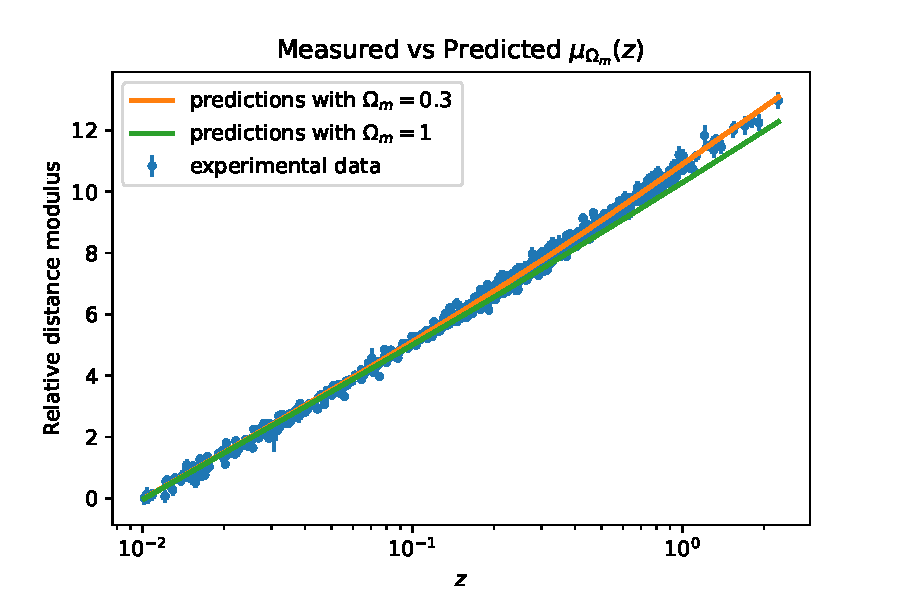
\includegraphics[width=1.1\textwidth]{img/sn_data.pdf}
    \caption{Comparison between observed and predicted SN Ia distance moduli assuming either $\Omega_m=0.3$ or $\Omega_m=1$, as function of redshift $z$. All $\mu$ values are expressed relative to the $\mu(z=0)$, i.e. we plot $\mu(z)/\mu(0)$.}
    \label{fig:sn_data}
\end{figure}
By looking at figure \ref{fig:sn_data} it appears that modifying the value of $\Omega_m$ does affect the predictions for $\mu(z)$, but not by much; indeed both values seem to be compatible with the available data (although $\Omega_m=0.3$ works a bit better at high $z$ values). 
In order to use this data to claim that dark energy exists we need to use Bayesian inference; what we need to prove, in particular is either that $\Omega_m$ is different from 1 in a cosmological model where the existence of dark energy is possible, or that such a model is much more credible than one without dark energy (at least according to this data).
The first option corresponds to Bayesian parameter inference, while the second one to Bayesian model selection; let us start from the first one, which is easier to implement.

We start by noting that the observed values for $\mu$ are distributed according to a Gaussian likelihood \cite{dark_energy_data} \cite{modern_cosmology}, which means that the log-likelihood is a simple quadratic form:
\begin{equation*}
    \ln\L \left(\vb*{\mu} | \hat{\vb*{\mu}}, \vb*{\Sigma}\right) = -\frac{1}{2}\left(\vb*{\mu}-\hat{\vb*{\mu}}\right)^T \vb*{\Sigma}^{-1}\left(\vb*{\mu}-\hat{\vb*{\mu}}\right)
\end{equation*}
where $\vb*{\mu}$ is the vector containing the observed values, $\hat{\vb*{\mu}}$ is the vector of predictions computed using eq. \eqref{eq:formula_luminosity_distance}, and the covariance matrix $\vb*{\Sigma}$ can be estimated using simulations and data from \cite{dark_energy_data}. Notice that we have ignored the parameter-independent normalization factor for simplicity, as we will normalize the distribution exactly later on.

Notice that, as said before, since we do not know the zero point for $\mu$, still ignoring the Gaussian normalization we pre-marginalize the likelihood over a constant additive value $\alpha = 5\log_{10} D_0$:
\begin{equation*}
    \L_m \left(\vb*{\mu} | \hat{\vb*{\mu}}, \vb*{\Sigma}\right) = \int \L \left(\vb*{\mu} | \hat{\vb*{\mu}}, \vb*{\Sigma}\right) \dd{\alpha} = \int \exp \left(-\frac{1}{2}\left(\vb*{\mu}-\hat{\vb*{\mu}} + \alpha\right)^T \vb*{\Sigma}^{-1}\left(\vb*{\mu}-\hat{\vb*{\mu}} + \alpha\right)\right) \dd{\alpha}
\end{equation*}
This allows us to rigorously account for the nuisance parameter $D_0$: thanks to marginalization we can take into account the uncertainty over this quantity. 

This integral can be solved exactly; it can be shown that the result is given by:
\begin{equation}
\label{eq:marginalized_likelihood}
    \ln \L_m\left(\vb*{\mu} | \hat{\vb*{\mu}}, \vb*{\Sigma}\right) =  -\frac{1}{2}\left(\vb*{\mu}-\hat{\vb*{\mu}}\right)^T \vb*{\Sigma}^{-1}\left(\vb*{\mu}-\hat{\vb*{\mu}}\right) + \frac{1}{2}\frac{\left[\vb{1}^T\vb*{\Sigma}^{-1}(\vb*{\mu}-\hat{\vb*{\mu}})\right]^2}{\vb{1}^T \vb*{\Sigma}^{-1} \vb{1}}
\end{equation}
where $\vb{1}$ is a vector of ones.

Equation \eqref{eq:marginalized_likelihood} gives us the likelihood we need to perform Bayesian inference; in order to use it we only need to compute the theoretical prediction $\hat{\vb*{\mu}}_{\Omega_m}(z)$ using the integral in equation \eqref{eq:formula_distance_modulus}, which can be easily solved numerically for any $\Omega_m \in [0, 1]$. Notice that, when solving this integral, we can safely ignore the $D_0$ constant thanks to the above marginalization.
The $\vb*{\mu}$ vector in equation \eqref{eq:marginalized_likelihood} is fixed, as it contains the measured values from \cite{dark_energy_data}; the same is true for $\vb*{\Sigma}$, which is estimated once and for all from the same data (and in our case has once again been taken from \cite{dark_energy_data}).

\subsubsection{A Computational Trick}
Before proceeding let us discuss a simple trick that can accelerate the numerical evaluation of the integral in \eqref{eq:formula_distance_modulus}.
The dataset used in this section is taken from \cite{dark_energy_data}, and consists of pairs $\{z_n, \mu(z_n)\}$: it is a sequence of redshift values whose corresponding distance modulus has been computed. 
Indeed we remark that what the authors of \cite{dark_energy_data} essentially did was observing a large number of supernovae, each at a certain redshift $z_n$, and measuring the distance modulus $\mu(z_n)$ of each supernova. In practice this means sampling from the likelihood in \eqref{eq:marginalized_likelihood} \emph{at redshift $z=z_n$}. For this reason in order to use this dataset to perform inference we must evaluate \eqref{eq:marginalized_likelihood} exactly on the sequence $\{z_n\}$; this means we need to evaluate \eqref{eq:formula_distance_modulus} in each of these redshift values, i.e. we have to compute the integrals $\int_0^{z_1}$, $\int_0^{z_2}$, $\int_0^{z_3}$, and so on. Assuming the $\{z_n\}$ sequence is sorted (i.e. $z_1<z_2<z_3<\dots$) this means these integrals are computed over intervals all starting from 0 and gradually increasing in size on the right; since the integrand function is always the same this allows us to simplify the numerical evaluation of these integrals.
To see why this is true let us start by computing the first integral, i.e. $\int_0^{z_1}$; then the second integral can be rewritten as $\int_0^{z_2} = \int_0^{z_1} + \int_{z_1}^{z_2}$ by exploiting the properties of integrals and the fact that $0<z_1<x_2$ by construction.
Similarly we can rewrite $\int_0^{z_3}$ as $\int_0^{z_1} + \int_{z_1}^{z_2} + \int_{z_2}^{z_3}$, and so on; in general if $I(n_1, n_2)$ is the integral between $z_{n_1}$ and $z_{n_2}$ we have that
\begin{equation*}
    \int_0^{z_n} = \sum_{i=2}^n I(i-1, i)
\end{equation*}
Let us say that we computed a vector containing all possible $I(i-1, i)$ values, i.e. a vector of the same integrals as in eq. \eqref{eq:formula_distance_modulus} \emph{but with bounds equal to consecutive redshift values}; then the integral from $0$ to any $z_n$ (and therefore any $\mu(z_n)$) can be computed by simply summing the first $n$ elements of this vector. Therefore the \emph{cumulative sum} of this vector will return the vector containing all $\mu(z_n)$ values corresponding to the given $\{z_n\}$ sequence.
Actually computing the theoretical predictions for the distance moduli in this way is not only equivalent, but also \emph{faster}: \emph{thanks to this approach we can compute $N$ integrals over smaller intervals}, instead of computing $N$ integrals of the same function over larger and larger intervals. Considering that numerical solvers need to evaluate the integrand between the given bounds this means that less steps overall are needed. 

To recap: the integrals we need to compute are over \emph{nested intervals}, in the sense that the first interval is contained in the second, the second in the third, and so on; this is due to the fact that they all have 0 as the lower bound, whereas the upper bounds are given by a monotonically increasing sequence $\{z_n\}$. This means that the integral from 0 $z_n$ is equal to the sum of the integrals between 0 and $z_1$, $z_1$ and $z_2$, and so on up to $z_{n-1}$ and $z_n$; therefore due to the properties of integrals the integral between 0 and $z_n$ is simply the sum of integrals all the consecutive redshift values smaller than the current one. Therefore instead computing $N$ integrals between $0$ and $z_n$ we can compute $N$ integrals between $z_{n-1}$ and $z_n$; by computing the cumulative sum of this second vector the result will be the same as the first one - with the useful advantage that, since the new integrals are computed over smaller intervals, each numerical evaluation is faster.
This trick has been implemented in the code used in this example to further speed up the whole execution.


\subsection{Inferring $\Omega_m$ With \textsc{CosmoLIME}}
We can now perform a Bayesian inference of $\Omega_m$ using the likelihood \eqref{eq:marginalized_likelihood} and the data and covariance matrix from \cite{dark_energy_data}.
By applying Bayes' theorem we obtain the posterior over $\Omega_m$:
\begin{equation*}
    P(\Omega_m|\{z_n, \mu(z_n)\}) \propto \L(\{z_n, \mu(z_n)\}|\Omega_m) P(\Omega_m)
\end{equation*}
where $D = \{z_n, \mu(z_n)\}$ is our dataset from \cite{dark_energy_data}, consisting of pairs of redshift values and the distance moduli measured at that redshift.
By ignoring the normalization factor (which will be addressed later) and taking logarithms we can write:
\begin{equation*}
    \ln P(\Omega_m|\{z_n, \mu(z_n)\}) = \ln\L(\{z_n, \mu(z_n)\}|\Omega_m) + \ln P(\Omega_m)
\end{equation*}
The log-likelihood term in the previous equation has already been computed in eq. \eqref{eq:marginalized_likelihood}, therefore we simply need to pick a log-prior  $\ln P(\Omega_m)$. For simplicity we can choose a flat i.e. uniform prior between two values $a$ and $b$:
\begin{equation*}
    P(\Omega_m) = 
    \begin{cases}
        \frac{1}{b-a} \ \ \text{if} \ a\leq \Omega_m\leq b\\
        0 \ \ \text{otherwise}
    \end{cases}
\end{equation*}
If $\Omega_m$  was an generic parameter we would have to arbitrarily choose the values for $a$ and $b$, but we can easily prove that there are physical requirements ensuring that $a=0$ and $b=1$. Indeed by definition $\Omega_m$ is a \emph{normalized density}; this means that it is a positive quantity that cannot be larger than 1, therefore the minimum value possible for $a$ is 0 and the maximum value possible for $b$ is 1. Of course we could a sub-interval in $[0, 1]$, such as e.g. $[0.2, 0.7]$, but we choose the widest possible prior to make it as uninformative as possible (while still describing only physical values of $\Omega_m$). This has the added benefit that prior volume is 1, i.e. $b-a=1$; this is useful because for example it means that $\ln P(\Omega_m) = 0$ in the above equation, which implies that the final posterior can be obtained simply by normalizing the exponential of the log-likelihood in eq. \eqref{eq:marginalized_likelihood}.

With this choice of the prior, then, the only remaining thing we have to do is to numerically evaluate the log-likelihood on the sequence $\{z_n\}$ by comparing the value \emph{observed} at $z_n$ and the value \emph{predicted} at $z_n$; computing the $N$ predictions needed for the $\{z_n\}_{n=1}^N$ sequence requires numerically solving the integral \eqref{eq:formula_distance_modulus} $N$ times (we already accelerated these numerical computations using the computational trick described in the previous section).

Notice that the $N$ integrals that need to be computed are \emph{not} a function of the dataset (which is fixed: $\{(z_n, \mu(z_n))\}$), but of the free parameter $\Omega_m$; this means that we can evaluate the posterior in any $\Omega_m$ value simply by adjusting the parameter in the denominator of \eqref{eq:formula_distance_modulus}.

To obtain the posterior numerically, therefore, what we can do is to e.g. define a linearly spaced grid of $\Omega_m$ values between 0 and 1 (the min. and max. values allowed by the prior), then compute the required integrals using the $\Omega_m$ values in this grid.
Evaluating the posterior on e.g. a grid of 1000-2000 points requires a few minutes; this means that this problem is simple enough that we can actually perform an exact inference from start to finish in just a few minutes.
In spite of this we now assume that the full posterior evaluation requires much longer, so much so that using an emulator may be beneficial; for this reason we may want to use \textsc{CosmoLIME} to replace the exact formula in \eqref{eq:marginalized_likelihood} with an approximated version, predicted using a machine learning model. Of course this example is simple enough that \textsc{CosmoLIME} is not really required, but we pretend it is to showcase its functionality in a true parameter inference pipeline.
Also notice that having access to a cheap exact likelihood means we can easily compare the predictions made by its exact and approximated versions; this is not only interesting, but actually necessary. Indeed as observed several times machine learning metrics can be deceiving; the true test of an emulator's performance is its ability to recover the correct (e.g. unbiased) posterior.
For this reason from now on we will perform calculations with the exact \emph{and} the emulated likelihood side-by-side.

We start by recovering the full posterior, e.g. by evaluating it on a linearly spaced grid of $\Omega_m$ values between 0 and 1. The exact posterior can be obtained using the numerical evaluations previously discussed; the emulated one requires using \textsc{CosmoLIME} to design an emulator satisfying the required characteristics.
To do so since this problem is very simple we can use a decision tree regressor; this will ensure an almost instantaneous optimization of the hyperparameters, while still returning an accurate predictor.
We can choose to optimize the same hyperparameters as in the previous examples; the main difference is that this time we set the much higher threshold of $R^2 = 99.998\%$; this is reasonable, because the posterior at hand is one dimensional and (as we will see in a moment) very close to a Gaussian, which means that it is trivial to emulate. This means that, unless the target is very high, \textsc{CosmoLIME} will settle on generating a small number of values; this may lead to inaccuracies in the inference pipeline, especially if we want to evaluate the posterior at high resolution i.e. using a really fine grid. To further prevent this issue we can ask \textsc{CosmoLIME} to generate a relatively high number of values in the first batch, like for example 1500 samples; these points are obtained using the same numerical integration needed to evaluate \eqref{eq:marginalized_likelihood} - which makes sense, considering we are trying to emulate the log-likelihood.
Using the code discussed in section \ref{sec:dark_energy_codes} the implementation of this emulation can be carried out in a couple of minutes.

After this is done we can evaluate the log-likelihood either exactly or by predicting its values using the freshly-built emulator (which, with for out particular choice of the seeds, reaches a final validation score $R^2\approx 99.9984\%$).

\begin{figure}[H]
    \centering
    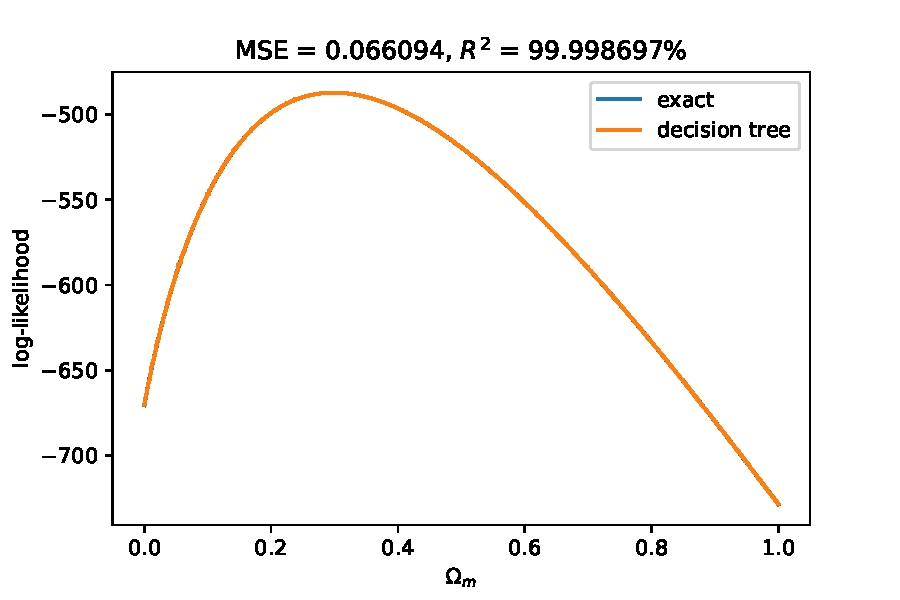
\includegraphics[width=1.0\textwidth]{img/loglikelihood_dt.pdf}
    \caption{Comparison between the log-likelihoods (as functions of $\Omega_m$) computed with and without the obtained emulator.}
    \label{fig:loglikelihood_dt}
\end{figure}

The two functions look basically indistinguishable; this is confirmed by the low MSE and by the $R^2\approx 1$ score.
By computing the exponential of the above values we can obtain the unnormalized posterior resulting from our choice of the prior.
Due to the fact that the values in the above plot are negative and with large absolute values simply taking the exponential will return an unnormalized posterior whose values are quite small; for simplicity we can divide the resulting posterior by its max. value, so that the peak of the posterior is located at a height equal to exactly 1 - which also ensures the other points have more practical values.

\begin{figure}[H]
    \centering
    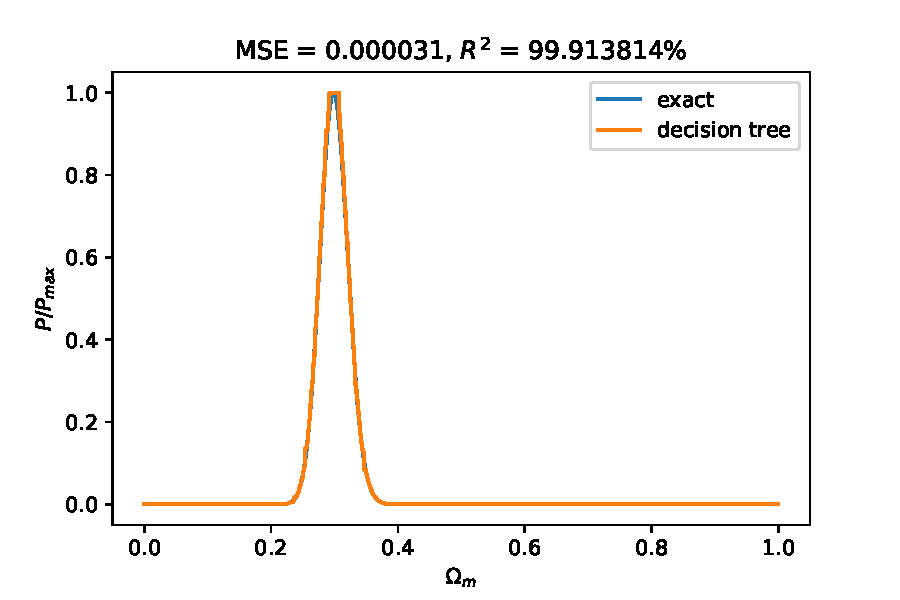
\includegraphics[width=1.0\textwidth]{img/posterior_dt.pdf}
    \caption{Comparison between the posteriors (normalized w.r.t. the max. values) computed with and without the obtained emulator.}
    \label{fig:posterior_dt}
\end{figure}
Once again the results are almost indistinguishable; the peaks are slightly different, and although this is barely noticeable we have to conclude that a great log-likelihood emulation turns into a slightly worse posterior emulation - which in any case is still quite good. This slight decrease in performance is confirmed by the $R^2$ score, which has decreased to $\sim 99.91\%$ - still quite good, which agrees with our qualitative conclusions. Interestingly enough the MSE has significantly decreased; this is a good example of the fact that machine learning metrics are not always reliable when it comes to evaluating an emulator's performance, which is why caution must be exercised and further tests performed.

Whether we use the exact or emulated likelihood we reach the same conclusion: \emph{the supernovae data at hand constrain the $\Omega_m$ parameter to $\sim 30\%$}. This inevitably implies that \emph{dark energy exists}, and that it must account for $\sim 70\%$ of all the ``stuff'' in the universe. 
This is a remarkable result; simply by observing figure \ref{fig:sn_data} we would have never guessed that the data constrains the model so strongly. Indeed even though we started with a flat prior (i.e. deemed all possible $\Omega_m$ values equally as believable) we end up with a very narrow peak, centered around $\Omega_m\approx 0.3$.

To recap: \emph{by fitting the model to the data we found a strong preference for $\Omega_m\approx 0.3$, with e.g. $\Omega_m\approx 1$ having negligible posterior probability; this proves the existence of dark energy, and that it represents about 70\% of the total cosmic inventory}.

\subsubsection{Posterior Normalization}
The posterior used above was not properly normalized, just divided by its max. value; in order to obtain the true posterior we need to normalize it by computing the \emph{evidence} and dividing the unnormalized posterior by this value. If we only care about e.g. the general shape of the posterior and/or the position of its peak (e.g. to compute the MAP estimator) this is not necessary, but it becomes mandatory if we want to use the posterior to compute actual probabilities (e.g. to obtain credibility intervals). 
In general computing the evidence is an intimidating task, but in our simple one dimensional example we can obtain it via direct numerical integration. The result, as we will see below, is a tiny number - and so are the values of the unnormalized posterior; for this reason a direct division leads to error or wrong results due to numerical precision issues. To avoid this we can perform an indirect division; in particular we can compute the difference between the log posterior and the log evidence, then compute the exponential. Due to the properties of logarithms and exponentials it is obvious that this operation is mathematically equivalent, but since the difference is more numerically stable than the division it works much better in practice. 
For this same reason (i.e. the evidence is a tiny number) later on we will report the value of the log evidence; this is a standard practice in situations like these.

\subsubsection{Summary Statistics}
Technically once the posterior has been obtained the whole inference is over; in Bayesian statistics the posterior contains a complete representation of all the information that can be learned by the data at hand, assuming a certain choice of the prior. In order to compress this information, though, we can compute some summary statistics; these are useful because they are easier to interpret at a glance, them being simply numbers.

\paragraph{Mean}
The posterior mean can be computed by numerically evaluating its definition:
\begin{equation*}
    \expval{\Omega_m} = \int_0^1 \Omega_m P(\Omega_m|D) \dd{\Omega_m}
\end{equation*}
The above definition can be used with the exact or emulated posteriors; we can compare the results using e.g. the MSE (mean squared error) or the MAE (mean absolute error), which in the case of just two numbers essentially means computing either the absolute value difference or the difference squared. We can also compute the relative error performed by using the emulator, which can be obtained by dividing the absolute value difference by the exact value.

We find:
\begin{verbatim}
mean_true = 0.29970000037102423, mean_emulator = 0.2997069133345322
MSE: 4.778906446246494e-11
MAE: 6.912963507965664e-06
rel. error: 2.3066277942634354e-05
\end{verbatim}

The estimate of the mean obtained using the emulator is accurate to 5 decimal places, and its relative error compared to the true value is of order $10^{-5}$; clearly the emulator is quite good.

\paragraph{Variance And Standard Deviation}
The posterior variance can be computed by numerically evaluating its definition:
\begin{equation*}
    \mathrm{Var} \ {\Omega_m} = \int_0^1 \left(\Omega_m - \expval{\Omega_m}\right)^2 P(\Omega_m|D) \dd{\Omega_m}
\end{equation*}
We find:
\begin{verbatim}
variance_true = 0.00048174813322270126, variance_emulator = 0.00048175929314920717
MSE: 1.2454395961739795e-16
MAE: 1.1159926505913825e-08
rel. error: 2.316547950327987e-05
\end{verbatim}
By taking the square root we can compute the standard deviation:
\begin{verbatim}
std_true = 0.021948761541888902, std_emulator = 0.021949015767209406
MSE: 6.463051358508387e-14
MAE: 2.542253205034539e-07
rel. error: 1.1582672672363244e-05
\end{verbatim}
Once again we find that the emulator's estimates are quite accurate.

By inspecting figure \ref{fig:posterior_dt} it becomes obvious that the final posterior is a Gaussian distribution, as expected; we can confirm this numerically by plotting an exact Gaussian defined by the same mean and variance as the true posterior. This essentially means approximating the posterior with a Gaussian with the same mean and variance; since we have just obtained these two values we can quickly check that the posterior and its Gaussian approximation are identical.
\begin{figure}[H]
    \centering
    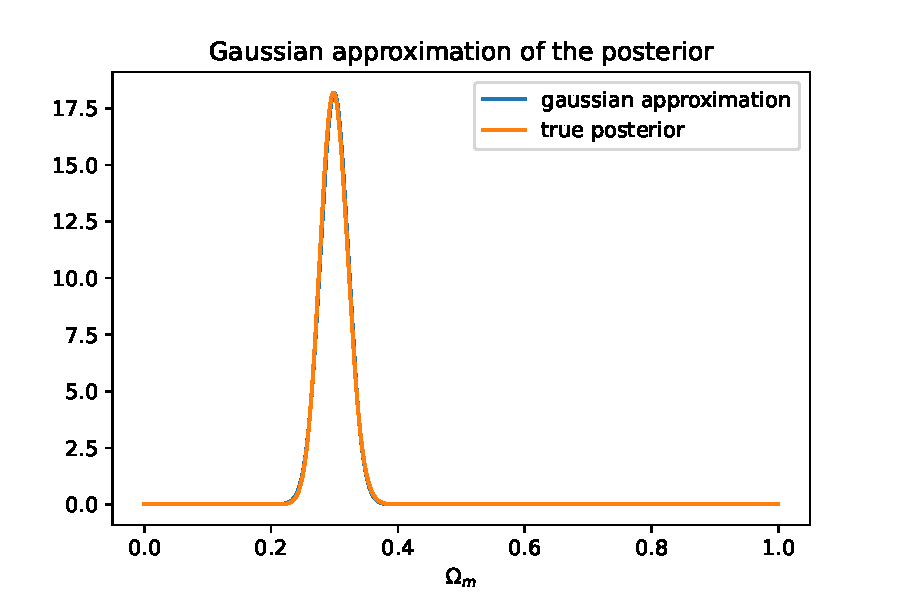
\includegraphics[width=\textwidth]{img/gaussian_approx.pdf}
    \caption{Gaussian approximation of the posterior: we plot the posterior and the Gaussian with the same mean and variance. They are clearly identical, which means that the obtained posterior is indeed a Gaussian distribution.}
\end{figure}

\paragraph{MAP}
A common Bayesian summary statistics is the MAP (maximum a posterior) estimator, i.e. the value of the parameter that maximizes the posterior. This is the value with maximum posterior probability, i.e. the most credible value; in our case it geometrically corresponds to the horizontal coordinate of the posterior's peak.

We find:
\begin{verbatim}
MAP_true = 0.2982982982982983, MAP_emulator = 0.2982982982982983
MSE: 0.0
MAE: 0.0
\end{verbatim}
In this case there is no difference between the true and emulator values; considering how common this estimator is this is very good news, as it means that the peak's position's emulator estimate is \emph{unbiased}.
We also remark that this value is almost identical to the mean due to the symmetry of the distribution (which as shown is essentially a Gaussian); the tiny difference between the two is probably mostly due to numerical precision issues.

\paragraph{Evidence}
As said before this example is simple enough that the evidence can be computed by direct numerical integration. In practice the computed evidence is a tiny number, which means it is best to work with its logarithm; in this way we can perform numerically stable operations, while also having a number that is easier to interpret.

We find:
\begin{verbatim}
log_evidence_true = -490.0910825817117, 
log_evidence_emulator = -490.0911056477236
MSE: 5.32040905895268e-10
MAE: 2.3066011920036544e-05
rel. error: -4.706474518681087e-08
\end{verbatim}


\paragraph{Credibility Intervals}
We now exploit the fact that we properly normalized the posterior, and can therefore compute probabilities. In particular we now compute \emph{credibility intervals}, i.e. the intervals that have $x\%$ posterior probability. This is equivalent to stating that we are $x\%$ sure that the parameter resides in the $x\%$ credibility interval; being able to rigorously use intuitive concepts like these is one of the main advantages of using a Bayesian approach.
Common values for credibility intervals mimic the $1\sigma$, $2\sigma$ and $3\sigma$ confidence levels of frequentist statistics, i.e. correspond to $68\%$, $95\%$ and $99\%$ probability; we find:
\begin{verbatim}
68% credibility interval (true and emulator):
[0.25725726 0.34334334] [0.25725726 0.34334334]
65% credibility interval difference:
[0. 0.]

95% credibility interval (true and emulator):
[0.25725726 0.34334334] [0.25725726 0.34334334]
95% credibility interval difference:
[0. 0.]

99% credibility interval difference:
[0.25725726 0.34334334] [0.25725726 0.34334334]
99% credibility interval difference:
[0. 0.]
\end{verbatim}
Similarly to the case of the MAP estimator we find no difference between the exact and emulator-based predictions. This is great news, because a common practice is to report parameter estimates as MAP $\pm$ credibility range; since these values are identical we can say that, from this point of view, \emph{the emulator provides with a perfectly accurate estimate of the posterior}. Indeed we just found that the results of these summary statistics are the same whether or not we use the emulator; in a realistic problem it would be the best possible result - assuming we are content with just this summary estimate of the parameter. The rest of the information that can be extracted from the posterior (including the posterior itself) has tiny differences between the exact and emulator-based predictions, but considering how tiny these are we can consider our emulator a success.

\begin{figure}[H]
    \centering
    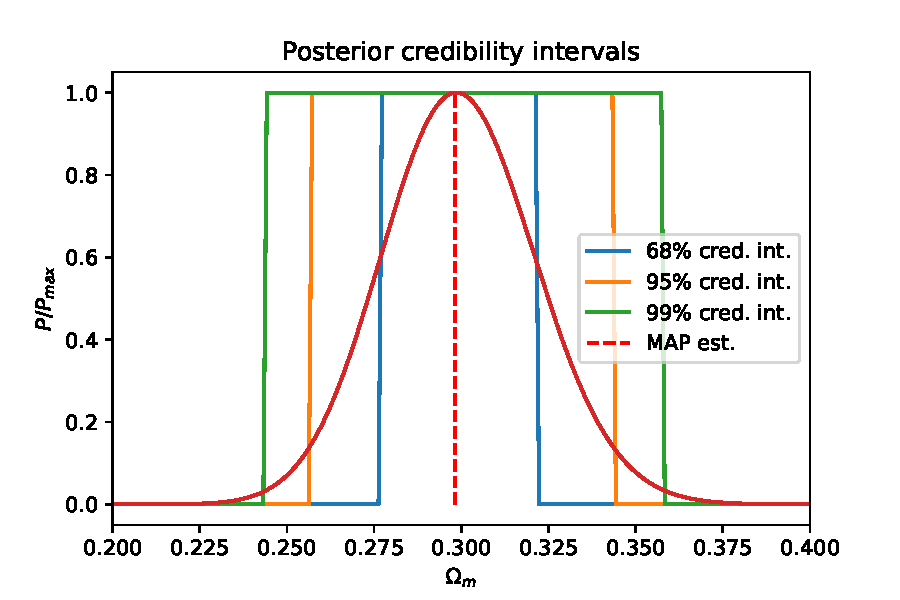
\includegraphics[width=\textwidth]{img/cred_intervals.pdf}
    \caption{Graphical representation of posterior credibility intervals.}
\end{figure}

To recap our inference we can use the MAP $\pm$ credibility intervals to report a final estimate of the parameter.
We found:
\begin{equation*}
    \Omega_m = 0.298 \pm 0.043 \ \ \ \text{($68\%$ cred. int.)}
\end{equation*}
This means that, after seeing this data, we are led to believe that dark energy exists, and represents $\sim 70\%$ of the total ``stuff'' in the universe.
Notice that these estimates are in line with the current best estimates; see for example \cite{dark_energy_data}.


\subsection{Bayesian Comparison Between the $\Omega_m=1$ and $\Omega_m\neq 1$ Models}
In the previous section we saw that one way to prove the existence of dark energy is to use a model where $\Omega_m$ is allowed to deviate from 1 (so that $\Omega_{\text{DE}}$ can be nonzero), then infer its value from some data.

Another possible approach is to perform \emph{Bayesian model comparison}; this second approach relies on comparing two whole models, i.e. ``there is no dark energy'' and ``there may be some dark energy''. This has the advantage of marginalizing out the model parameters; indeed we can assign a posterior probability to the whole model \emph{irrespective of its distribution over parameters}.
To see how this may be performed in practice we briefly summarize the main results regarding Bayesian model selection/comparison; the following discussion is based on \cite{mckay}.

\subsubsection{Model Comparison Summary}
Assume we have a certain number of models $M_i$, each with its own parameters; if we could assign a \emph{posterior probability} to them (after seeing some data) then we could compare them, e.g. to understand which model is more credible according to the available data.
The great thing about Bayes' theorem is that it can be applied to \emph{anything}; we can therefore use it to assign a posterior probability to our set of models $\{M_i\}$:
\begin{equation*}
    P(M_i|D) = \frac{P(D|M_i) P(M_i)}{P(D)}
\end{equation*}
The term in the denominator is simply the normalization constant of the numerator, and can be obtained as $P(D) = \sum_i P(D|M_i) P(M_i)$; as long as we only care about ratios of posterior probabilities (e.g. to compare two models) we can safely ignore this quantity. Similarly the $P(M_i)$ term can be safely ignored, as it simply represents the prior probability assigned to different models - which we often set to a uniform prior.

We are left with $P(D|M_i)$, which is exactly the \emph{evidence} term we would obtain by performing simple parameter inference with model $M_i$; therefore model selection can be performed using ``recycled'' results from parameter inference.\footnote{As said before the evidence is usually very expensive to compute, but once it is computed it can be used to perform model selection; in any case this is not an issue in our simple example, where the evidence can be immediately obtained by direct numerical integration.}
Therefore assigning posterior probabilities in practice hinges on computing the quantity
\begin{equation*}
    P(D|M_i) = \int \dd{\theta} P(D|\theta, M_i) P(\theta|M_i)
\end{equation*}
where $\theta$ is the (set of) model's parameter(s).
The interesting thing about this quantity is that \emph{it automatically ensures Bayesian model comparison follows Occam's principle}, which is the idea that the simplest possible explanation that can still explain the observation should probably be preferred.
To see why this is true let us consider a simple situation where we have a one-dimensional posterior with a strong peak, i.e. an approximately Gaussian 1D posterior. In this case the evidence can be approximated using Laplace's method, i.e. by multiplying the height of the peak of the integrand ($P(D|\theta_{\text{MP}}, M_i)$) by the posterior's width ($\sigma_{\theta|D}$):
\begin{equation*}
    P(D|M_i) \approx P(D|\theta_{\text{MP}}, M_i) \times P(\theta_{\text{MP}}|M_i)\sigma_{\theta|D}
\end{equation*}
Considering that $\theta_{\text{MP}}$ is the most probable value of $\theta$ we can rewrite the previous equation as follows:
\begin{equation*}
    \text{Evidence} \approx \text{Best fit Likelihood} \times \text{Occam factor}
\end{equation*}
where we called \emph{Occam factor} the $P(\theta_{\text{MP}}|M_i)\sigma_{\theta|D}$ term. This term is interesting because \emph{it penalizes the model complexity}, therefore preferring the simpler models (as stated by Occam's razor).
Let us discuss why this is true and why it matters

\paragraph{How The Occam Factor Penalizes Model Complexity}
Let us assume for simplicity that the prior $P(\theta|M_i)$ is uniform over a wide interval of length $\sigma_\theta$, representing the values of $\theta$ that are possible a priori. Then $P(\theta_{\text{MP}}|M_i) = 1/\sigma_\theta$, and we obtain that
\begin{equation*}
    \text{Occam factor} = \frac{\sigma_{\theta|D}}{\sigma_\theta}
\end{equation*}
This means that \emph{the Occam factor is equal to the ratio of the posterior accessible volume of $M_i$'s parameter space to the prior accessible volume, or equivalently the factor by which $M_i$'s hypothesis space collapses when the data arrive}. Indeed we observe that model $M_i$ can be viewed as consisting of a certain number of exclusive submodels, of which only one survives when the data arrive; the Occam factor is the inverse of this number. For this reason the accessible volume in parameter space shrinks when a dataset is observed, because some values that were possible a priori no longer are a posteriori.
By quoting from \cite{mckay} we learn why this is relevant:
\begin{quote}
A complex model having many parameters, each of which is free to vary over a large range $\sigma_\theta$, will typically be penalized by a stronger Occam factor than a simpler model. The Occam factor also penalizes models that have to
be finely tuned to fit the data, favouring models for which the required precision of the parameters $\sigma_{\theta|D}$ is coarse. The magnitude of the Occam factor is thus a measure of complexity of the model; it relates to the complexity of
the predictions that the model makes in data space. This depends not only on the number of parameters in the model, but also on the prior probability that the model assigns to them. Which model achieves the greatest evidence
is determined by a trade-off between minimizing this natural complexity measure and minimizing the data misfit. In contrast to alternative measures of model complexity, the Occam factor for a model is straightforward to evaluate: it simply depends on the error bars on the parameters, which we already evaluated when fitting the model to the data.
\end{quote}

A more complex model is one that can be fit accurately to a wide range of possible data, whereas a simpler one does not work as well as often. In our approximation this essentially means that a more complex model has a wider $\sigma_\theta$, i.e. the model a priori allows for a wider range of possible parameter values to ensure it can more accurately fit a broader set of possible data. This means that, once the data arrive, the accessible parameter volume (i.e. the range of parameter values that are still possible) shrinks much more, which means that the Occam factor is much smaller for a complex model than for a simple one. Therefore when computing the evidence what often happens in practice is that the evidence for more complex models is lower, due to the fact that the Occam factor itself is lower. This happens in spite of the fact that more complex models will always achieve a higher value of the best fit likelihood; indeed for a more complex model to be accepted it must be so much better than the simple model that it can overcome the penalization assigned by the Occam factor.


\paragraph{The Occam Factor From A Machine Learning Point of View}
In general by increasing the complexity of a model (e.g. by adding parameters) we can always improve how closely the model fits the data. Since this can always be done it seems that in principle one should always prefer more complex models; the issue with arbitrarily high model complexity is that too much of it can lead to overfitting, as stated multiple times. Indeed if a model learns too accurately the patterns inside data it can actually learn e.g. random noise fluctuations, causing it to performing terribly once new data arrives; this problem is called \emph{overfitting}, and is an issue because it causes a model to not generalize well to new data. Therefore (in agreement with Occam's principle) we should always look for a compromise between a accuracy and complexity, preferring the simplest possible model that still works reasonably well; as we saw above this model is more probable, and therefore has the best chance of generalizing well to new data. 
When using machine learning models one must artificially insert a term that penalizes model complexity to ensure this trade-off is respected; this can be challenging, because e.g. this extra term depends on an arbitrary choice. Using Bayesian model selection this problem solves itself: Occam's factor automatically takes into account model complexity when performing model comparison, so in order for a more complex model to be more probable it has to be so much better that it actually overcomes the penalization it receives due to being a more complex model.



\subsubsection{Proving The Existence of Dark Energy With Model Selection}
Having learned how evidence can be used to assign posterior probabilities to whole models we now apply this knowledge to our problem.
In order to understand whether dark energy exists or not we can compare the posterior probabilities assigned to a model without dark energy and a model with it; this essentially means comparing a model where $\Omega_m=1$ (i.e. there exists only matter) to one where $\Omega_m$ is allowed to be different from 1 (i.e. dark energy may exist, and we want to learn how much there is).

In order to compare these two models - which from now on we call $M_0$ and $M_1$ - we can compute the ratio of their posterior probabilities conditioned on the same supernova dataset $D$ as in the previous section:
\begin{equation*}
    \frac{P(M_1|D)}{P(M_0|D)} = \frac{P(D|M_1)P(M_1)}{P(D|M_0)P(M_0)}
\end{equation*}
where the $P(D)$ common term simplifies - hence why it makes sense to use this ratio. Assuming equal prior probabilities i.e. that a priori $M_0$ and $M_1$ are equally as credible the previous equation further simplifies:
\begin{equation*}
    \frac{P(M_1|D)}{P(M_0|D)} = \frac{P(D|M_1)}{P(D|M_0)}
\end{equation*}
i.e. the model posterior probability ratio is equal to the ratio of evidences; as stated before the evidence can then be used to rank the models' credibilities.

We remark that model $M_0$ has no free parameters, because it sets $\Omega_{\text{DE}} = 0$ and therefore $\Omega_m = 1$; model $M_1$, instead, has one free parameter (either $\Omega_{\text{DE}}$ or $\Omega_m$) that is allowed to vary. This means that model $M_1$ is more complex, and will therefore be penalized by the Occam factor; if in spite of this it turns out that it is still favored then it truly means that a universe with dark energy is more credible than one without it.

Let us now compute the two evidences to settle this matter.
\paragraph{Evidence of model $M_1$}
The evidence of model $M_1$ has to keep into account that this time $\Omega_m$ can vary freely between 0 and 1; therefore in this case the evidence must be computed as the normalization factor of the $\Omega_m$ posterior, i.e. the denominator in Bayes' theorem:
\begin{equation*}
    E_1 = P(D|M_1) = \int_0^1 \dd{\Omega_m} P(D|\Omega_m, M_1) P(\Omega_m|M_1)
\end{equation*}
This quantity has already been numerically evaluated in the previous section, therefore is already known.


\paragraph{Evidence of model $M_0$}
By definition $M_0: \Omega_m = 1$, as this model describes a universe with no dark matter. 
\begin{comment}
Since $M_0$ is equivalent to the case where $\Omega_m = 1$ we can simply write:
\begin{equation*}
    P(M_0|D) = P(\Omega_m = 1|D)
\end{equation*}
from which it immediately follows that \emph{the evidence of model $M_0$ is simply the $\Omega_m$ posterior evaluated at $\Omega_m = 1$}.
\end{comment}
This means that $P(\Omega_m|M_0) = \delta(\Omega_m-1)$, i.e. the only value that is allowed a priori is $\Omega_m = 1$.
By substituting this in the definition of the evidence we find:
\begin{equation*}
    E_0 = P(D|M_0) = \int_0^1 \dd{\Omega_m} P(D|\Omega_m, M_0) P(\Omega_m|M_0) = 
\end{equation*}
\begin{equation*}
    = \int_0^1 \dd{\Omega_m} P(D|\Omega_m, M_0) \delta(\Omega_m - 1) = P(D|\Omega_m = 1)
\end{equation*}
Since we chose a uniform prior when dealing with model $M_1$ we found that the likelihood and the posterior were equal; combining this with the previous result we obtain that \emph{the evidence $E_0$ is equal to $P(\Omega_m=1|D)$}, i.e. the posterior evaluated in $\Omega_m = 1$. This makes sense: since model $M_0$ is equivalent to a specific submodel of $M_1$ it seems reasonable that the overall probability we assign to $M_0$ can be computed as the probability of a specific realization of model $M_1$.

By working with the log evidences we can compute the ratio of evidence and posterior in $\Omega_m = 1$ as the difference between the log evidence and the log posterior. By doing so we obtain the value \texttt{238.58804160030934} (irrespectively of whether or not we use the emulator), which means that \emph{the model with dark energy is strongly preferred}, so much so that despite its increased complexity it can strongly overcome the penalization induced by the Occam factor. Said in another way this results shows that the improvement in the fit of the Dark Energy model with respect to the matter only model is largely overcoming Occam's skepticism.

\subsection{Summary of Results}
By using Bayesian parameter inference and model comparison we found out that \emph{the universe cannot be made up of only matter}; in particular we found that (dark) matter can at most be $\sim 30\%$ of the total cosmic inventory. This means that $70\%$ of the ``stuff'' in the universe is unaccounted for; we call this extra ``stuff'' \emph{dark energy}.

This example was of course very simplified, but still based on true experimental data; also the conclusions we reached are consistent with the commonly accepted standard model of cosmology.
Finally we remark that this example shows how easy \textsc{CosmoLIME} can fit into pre-existing inference pipelines; indeed by simply replacing a single part everything still works in the same way - provided the correct statistical checks are performed; this example also served to show how this may be done in practice, too.